\documentclass[twoside]{book}

% Packages required by doxygen
\usepackage{fixltx2e}
\usepackage{calc}
\usepackage{doxygen}
\usepackage[export]{adjustbox} % also loads graphicx
\usepackage{graphicx}
\usepackage[utf8]{inputenc}
\usepackage{makeidx}
\usepackage{multicol}
\usepackage{multirow}
\PassOptionsToPackage{warn}{textcomp}
\usepackage{textcomp}
\usepackage[nointegrals]{wasysym}
\usepackage[table]{xcolor}

% Font selection
\usepackage[T1]{fontenc}
\usepackage[scaled=.90]{helvet}
\usepackage{courier}
\usepackage{amssymb}
\usepackage{sectsty}
\renewcommand{\familydefault}{\sfdefault}
\allsectionsfont{%
  \fontseries{bc}\selectfont%
  \color{darkgray}%
}
\renewcommand{\DoxyLabelFont}{%
  \fontseries{bc}\selectfont%
  \color{darkgray}%
}
\newcommand{\+}{\discretionary{\mbox{\scriptsize$\hookleftarrow$}}{}{}}

% Page & text layout
\usepackage{geometry}
\geometry{%
  a4paper,%
  top=2.5cm,%
  bottom=2.5cm,%
  left=2.5cm,%
  right=2.5cm%
}
\tolerance=750
\hfuzz=15pt
\hbadness=750
\setlength{\emergencystretch}{15pt}
\setlength{\parindent}{0cm}
\setlength{\parskip}{3ex plus 2ex minus 2ex}
\makeatletter
\renewcommand{\paragraph}{%
  \@startsection{paragraph}{4}{0ex}{-1.0ex}{1.0ex}{%
    \normalfont\normalsize\bfseries\SS@parafont%
  }%
}
\renewcommand{\subparagraph}{%
  \@startsection{subparagraph}{5}{0ex}{-1.0ex}{1.0ex}{%
    \normalfont\normalsize\bfseries\SS@subparafont%
  }%
}
\makeatother

% Headers & footers
\usepackage{fancyhdr}
\pagestyle{fancyplain}
\fancyhead[LE]{\fancyplain{}{\bfseries\thepage}}
\fancyhead[CE]{\fancyplain{}{}}
\fancyhead[RE]{\fancyplain{}{\bfseries\leftmark}}
\fancyhead[LO]{\fancyplain{}{\bfseries\rightmark}}
\fancyhead[CO]{\fancyplain{}{}}
\fancyhead[RO]{\fancyplain{}{\bfseries\thepage}}
\fancyfoot[LE]{\fancyplain{}{}}
\fancyfoot[CE]{\fancyplain{}{}}
\fancyfoot[RE]{\fancyplain{}{\bfseries\scriptsize Generated by Doxygen }}
\fancyfoot[LO]{\fancyplain{}{\bfseries\scriptsize Generated by Doxygen }}
\fancyfoot[CO]{\fancyplain{}{}}
\fancyfoot[RO]{\fancyplain{}{}}
\renewcommand{\footrulewidth}{0.4pt}
\renewcommand{\chaptermark}[1]{%
  \markboth{#1}{}%
}
\renewcommand{\sectionmark}[1]{%
  \markright{\thesection\ #1}%
}

% Indices & bibliography
\usepackage{natbib}
\usepackage[titles]{tocloft}
\setcounter{tocdepth}{3}
\setcounter{secnumdepth}{5}
\makeindex

% Hyperlinks (required, but should be loaded last)
\usepackage{ifpdf}
\ifpdf
  \usepackage[pdftex,pagebackref=true]{hyperref}
\else
  \usepackage[ps2pdf,pagebackref=true]{hyperref}
\fi
\hypersetup{%
  colorlinks=true,%
  linkcolor=blue,%
  citecolor=blue,%
  unicode%
}

% Custom commands
\newcommand{\clearemptydoublepage}{%
  \newpage{\pagestyle{empty}\cleardoublepage}%
}

\usepackage{caption}
\captionsetup{labelsep=space,justification=centering,font={bf},singlelinecheck=off,skip=4pt,position=top}

%===== C O N T E N T S =====

\begin{document}

% Titlepage & ToC
\hypersetup{pageanchor=false,
             bookmarksnumbered=true,
             pdfencoding=unicode
            }
\pagenumbering{alph}
\begin{titlepage}
\vspace*{7cm}
\begin{center}%
{\Large Analyzer Code }\\
\vspace*{1cm}
{\large Generated by Doxygen 1.8.13}\\
\end{center}
\end{titlepage}
\clearemptydoublepage
\pagenumbering{roman}
\tableofcontents
\clearemptydoublepage
\pagenumbering{arabic}
\hypersetup{pageanchor=true}

%--- Begin generated contents ---
\chapter{Hierarchical Index}
\section{Class Hierarchy}
This inheritance list is sorted roughly, but not completely, alphabetically\+:\begin{DoxyCompactList}
\item \contentsline{section}{analyzer.\+code.\+Enum\+Mark\+Count\+Operators}{\pageref{enumanalyzer_1_1code_1_1EnumMarkCountOperators}}{}
\item \contentsline{section}{analyzer.\+code.\+Enum\+Mark\+Level\+Nest}{\pageref{enumanalyzer_1_1code_1_1EnumMarkLevelNest}}{}
\item \contentsline{section}{analyzer.\+code.\+Enum\+Mark\+Middle\+Len\+Ident}{\pageref{enumanalyzer_1_1code_1_1EnumMarkMiddleLenIdent}}{}
\item \contentsline{section}{analyzer.\+code.\+Enum\+Name\+MetricC}{\pageref{enumanalyzer_1_1code_1_1EnumNameMetricC}}{}
\item \contentsline{section}{analyzer.\+code.\+Enum\+Names\+Metric}{\pageref{enumanalyzer_1_1code_1_1EnumNamesMetric}}{}
\item \contentsline{section}{analyzer.\+code.\+Event}{\pageref{classanalyzer_1_1code_1_1Event}}{}
\item \contentsline{section}{analyzer.\+code.\+I\+Analayzer}{\pageref{interfaceanalyzer_1_1code_1_1IAnalayzer}}{}
\begin{DoxyCompactList}
\item \contentsline{section}{analyzer.\+code.\+AnalyzerC}{\pageref{classanalyzer_1_1code_1_1AnalyzerC}}{}
\end{DoxyCompactList}
\item \contentsline{section}{analyzer.\+code.\+I\+Calculate\+Mark}{\pageref{interfaceanalyzer_1_1code_1_1ICalculateMark}}{}
\begin{DoxyCompactList}
\item \contentsline{section}{analyzer.\+code.\+Calculate\+MarkC}{\pageref{classanalyzer_1_1code_1_1CalculateMarkC}}{}
\end{DoxyCompactList}
\item \contentsline{section}{analyzer.\+code.\+I\+Metric}{\pageref{interfaceanalyzer_1_1code_1_1IMetric}}{}
\begin{DoxyCompactList}
\item \contentsline{section}{analyzer.\+code.\+Count\+Operators}{\pageref{classanalyzer_1_1code_1_1CountOperators}}{}
\item \contentsline{section}{analyzer.\+code.\+Level\+Nesting}{\pageref{classanalyzer_1_1code_1_1LevelNesting}}{}
\item \contentsline{section}{analyzer.\+code.\+Middle\+Len\+Ident}{\pageref{classanalyzer_1_1code_1_1MiddleLenIdent}}{}
\end{DoxyCompactList}
\item \contentsline{section}{analyzer.\+code.\+Lexem}{\pageref{classanalyzer_1_1code_1_1Lexem}}{}
\item \contentsline{section}{analyzer.\+code.\+Listener}{\pageref{classanalyzer_1_1code_1_1Listener}}{}
\begin{DoxyCompactList}
\item \contentsline{section}{analyzer.\+code.\+Event\+Count\+Operator}{\pageref{classanalyzer_1_1code_1_1EventCountOperator}}{}
\item \contentsline{section}{analyzer.\+code.\+Event\+Level\+Nest}{\pageref{classanalyzer_1_1code_1_1EventLevelNest}}{}
\item \contentsline{section}{analyzer.\+code.\+Event\+Middle\+Len\+Ident}{\pageref{classanalyzer_1_1code_1_1EventMiddleLenIdent}}{}
\end{DoxyCompactList}
\item \contentsline{section}{analyzer.\+code.\+Metric\+Setting}{\pageref{classanalyzer_1_1code_1_1MetricSetting}}{}
\item \contentsline{section}{analyzer.\+code.\+Scaner}{\pageref{classanalyzer_1_1code_1_1Scaner}}{}
\begin{DoxyCompactList}
\item \contentsline{section}{analyzer.\+code.\+Scaner\+C\+Plus\+Plus}{\pageref{classanalyzer_1_1code_1_1ScanerCPlusPlus}}{}
\end{DoxyCompactList}
\item \contentsline{section}{analyzer.\+code.\+Syntax\+Analyzer}{\pageref{classanalyzer_1_1code_1_1SyntaxAnalyzer}}{}
\begin{DoxyCompactList}
\item \contentsline{section}{analyzer.\+code.\+Syntax\+Analyzer\+C\+Plus\+Plus}{\pageref{classanalyzer_1_1code_1_1SyntaxAnalyzerCPlusPlus}}{}
\end{DoxyCompactList}
\item \contentsline{section}{analyzer.\+code.\+Unknown}{\pageref{classanalyzer_1_1code_1_1Unknown}}{}
\item \contentsline{section}{analyzer.\+code.\+Variable}{\pageref{classanalyzer_1_1code_1_1Variable}}{}
\item Application\begin{DoxyCompactList}
\item \contentsline{section}{analyzer.\+code.\+Analyzer\+Code}{\pageref{classanalyzer_1_1code_1_1AnalyzerCode}}{}
\end{DoxyCompactList}
\item Initializable\begin{DoxyCompactList}
\item \contentsline{section}{analyzer.\+code.\+F\+X\+M\+L\+About\+Programm\+Controller}{\pageref{classanalyzer_1_1code_1_1FXMLAboutProgrammController}}{}
\item \contentsline{section}{analyzer.\+code.\+F\+X\+M\+L\+Analyzer\+Controller}{\pageref{classanalyzer_1_1code_1_1FXMLAnalyzerController}}{}
\item \contentsline{section}{analyzer.\+code.\+F\+X\+M\+L\+Metrics\+Controller}{\pageref{classanalyzer_1_1code_1_1FXMLMetricsController}}{}
\item \contentsline{section}{analyzer.\+code.\+F\+X\+M\+L\+Select\+Used\+Project\+Controller}{\pageref{classanalyzer_1_1code_1_1FXMLSelectUsedProjectController}}{}
\item \contentsline{section}{analyzer.\+code.\+F\+X\+M\+L\+Setting\+Controller}{\pageref{classanalyzer_1_1code_1_1FXMLSettingController}}{}
\end{DoxyCompactList}
\end{DoxyCompactList}

\chapter{Class Index}
\section{Class List}
Here are the classes, structs, unions and interfaces with brief descriptions\+:\begin{DoxyCompactList}
\item\contentsline{section}{\hyperlink{classanalyzer_1_1code_1_1AnalyzerC}{analyzer.\+code.\+AnalyzerC} }{\pageref{classanalyzer_1_1code_1_1AnalyzerC}}{}
\item\contentsline{section}{\hyperlink{classanalyzer_1_1code_1_1AnalyzerCode}{analyzer.\+code.\+Analyzer\+Code} }{\pageref{classanalyzer_1_1code_1_1AnalyzerCode}}{}
\item\contentsline{section}{\hyperlink{classanalyzer_1_1code_1_1CalculateMarkC}{analyzer.\+code.\+Calculate\+MarkC} }{\pageref{classanalyzer_1_1code_1_1CalculateMarkC}}{}
\item\contentsline{section}{\hyperlink{classanalyzer_1_1code_1_1CountOperators}{analyzer.\+code.\+Count\+Operators} }{\pageref{classanalyzer_1_1code_1_1CountOperators}}{}
\item\contentsline{section}{\hyperlink{enumanalyzer_1_1code_1_1EnumMarkCountOperators}{analyzer.\+code.\+Enum\+Mark\+Count\+Operators} }{\pageref{enumanalyzer_1_1code_1_1EnumMarkCountOperators}}{}
\item\contentsline{section}{\hyperlink{enumanalyzer_1_1code_1_1EnumMarkLevelNest}{analyzer.\+code.\+Enum\+Mark\+Level\+Nest} }{\pageref{enumanalyzer_1_1code_1_1EnumMarkLevelNest}}{}
\item\contentsline{section}{\hyperlink{enumanalyzer_1_1code_1_1EnumMarkMiddleLenIdent}{analyzer.\+code.\+Enum\+Mark\+Middle\+Len\+Ident} }{\pageref{enumanalyzer_1_1code_1_1EnumMarkMiddleLenIdent}}{}
\item\contentsline{section}{\hyperlink{enumanalyzer_1_1code_1_1EnumNameMetricC}{analyzer.\+code.\+Enum\+Name\+MetricC} }{\pageref{enumanalyzer_1_1code_1_1EnumNameMetricC}}{}
\item\contentsline{section}{\hyperlink{enumanalyzer_1_1code_1_1EnumNamesMetric}{analyzer.\+code.\+Enum\+Names\+Metric} }{\pageref{enumanalyzer_1_1code_1_1EnumNamesMetric}}{}
\item\contentsline{section}{\hyperlink{classanalyzer_1_1code_1_1Event}{analyzer.\+code.\+Event} }{\pageref{classanalyzer_1_1code_1_1Event}}{}
\item\contentsline{section}{\hyperlink{classanalyzer_1_1code_1_1EventCountOperator}{analyzer.\+code.\+Event\+Count\+Operator} }{\pageref{classanalyzer_1_1code_1_1EventCountOperator}}{}
\item\contentsline{section}{\hyperlink{classanalyzer_1_1code_1_1EventLevelNest}{analyzer.\+code.\+Event\+Level\+Nest} }{\pageref{classanalyzer_1_1code_1_1EventLevelNest}}{}
\item\contentsline{section}{\hyperlink{classanalyzer_1_1code_1_1EventMiddleLenIdent}{analyzer.\+code.\+Event\+Middle\+Len\+Ident} }{\pageref{classanalyzer_1_1code_1_1EventMiddleLenIdent}}{}
\item\contentsline{section}{\hyperlink{classanalyzer_1_1code_1_1FXMLAboutProgrammController}{analyzer.\+code.\+F\+X\+M\+L\+About\+Programm\+Controller} }{\pageref{classanalyzer_1_1code_1_1FXMLAboutProgrammController}}{}
\item\contentsline{section}{\hyperlink{classanalyzer_1_1code_1_1FXMLAnalyzerController}{analyzer.\+code.\+F\+X\+M\+L\+Analyzer\+Controller} }{\pageref{classanalyzer_1_1code_1_1FXMLAnalyzerController}}{}
\item\contentsline{section}{\hyperlink{classanalyzer_1_1code_1_1FXMLMetricsController}{analyzer.\+code.\+F\+X\+M\+L\+Metrics\+Controller} }{\pageref{classanalyzer_1_1code_1_1FXMLMetricsController}}{}
\item\contentsline{section}{\hyperlink{classanalyzer_1_1code_1_1FXMLSelectUsedProjectController}{analyzer.\+code.\+F\+X\+M\+L\+Select\+Used\+Project\+Controller} }{\pageref{classanalyzer_1_1code_1_1FXMLSelectUsedProjectController}}{}
\item\contentsline{section}{\hyperlink{classanalyzer_1_1code_1_1FXMLSettingController}{analyzer.\+code.\+F\+X\+M\+L\+Setting\+Controller} }{\pageref{classanalyzer_1_1code_1_1FXMLSettingController}}{}
\item\contentsline{section}{\hyperlink{interfaceanalyzer_1_1code_1_1IAnalayzer}{analyzer.\+code.\+I\+Analayzer} }{\pageref{interfaceanalyzer_1_1code_1_1IAnalayzer}}{}
\item\contentsline{section}{\hyperlink{interfaceanalyzer_1_1code_1_1ICalculateMark}{analyzer.\+code.\+I\+Calculate\+Mark} }{\pageref{interfaceanalyzer_1_1code_1_1ICalculateMark}}{}
\item\contentsline{section}{\hyperlink{interfaceanalyzer_1_1code_1_1IMetric}{analyzer.\+code.\+I\+Metric} }{\pageref{interfaceanalyzer_1_1code_1_1IMetric}}{}
\item\contentsline{section}{\hyperlink{classanalyzer_1_1code_1_1LevelNesting}{analyzer.\+code.\+Level\+Nesting} }{\pageref{classanalyzer_1_1code_1_1LevelNesting}}{}
\item\contentsline{section}{\hyperlink{classanalyzer_1_1code_1_1Lexem}{analyzer.\+code.\+Lexem} }{\pageref{classanalyzer_1_1code_1_1Lexem}}{}
\item\contentsline{section}{\hyperlink{classanalyzer_1_1code_1_1Listener}{analyzer.\+code.\+Listener} }{\pageref{classanalyzer_1_1code_1_1Listener}}{}
\item\contentsline{section}{\hyperlink{classanalyzer_1_1code_1_1MetricSetting}{analyzer.\+code.\+Metric\+Setting} }{\pageref{classanalyzer_1_1code_1_1MetricSetting}}{}
\item\contentsline{section}{\hyperlink{classanalyzer_1_1code_1_1MiddleLenIdent}{analyzer.\+code.\+Middle\+Len\+Ident} }{\pageref{classanalyzer_1_1code_1_1MiddleLenIdent}}{}
\item\contentsline{section}{\hyperlink{classanalyzer_1_1code_1_1Scaner}{analyzer.\+code.\+Scaner} }{\pageref{classanalyzer_1_1code_1_1Scaner}}{}
\item\contentsline{section}{\hyperlink{classanalyzer_1_1code_1_1ScanerCPlusPlus}{analyzer.\+code.\+Scaner\+C\+Plus\+Plus} }{\pageref{classanalyzer_1_1code_1_1ScanerCPlusPlus}}{}
\item\contentsline{section}{\hyperlink{classanalyzer_1_1code_1_1SyntaxAnalyzer}{analyzer.\+code.\+Syntax\+Analyzer} }{\pageref{classanalyzer_1_1code_1_1SyntaxAnalyzer}}{}
\item\contentsline{section}{\hyperlink{classanalyzer_1_1code_1_1SyntaxAnalyzerCPlusPlus}{analyzer.\+code.\+Syntax\+Analyzer\+C\+Plus\+Plus} }{\pageref{classanalyzer_1_1code_1_1SyntaxAnalyzerCPlusPlus}}{}
\item\contentsline{section}{\hyperlink{classanalyzer_1_1code_1_1Unknown}{analyzer.\+code.\+Unknown} }{\pageref{classanalyzer_1_1code_1_1Unknown}}{}
\item\contentsline{section}{\hyperlink{classanalyzer_1_1code_1_1Variable}{analyzer.\+code.\+Variable} }{\pageref{classanalyzer_1_1code_1_1Variable}}{}
\end{DoxyCompactList}

\chapter{Class Documentation}
\hypertarget{classanalyzer_1_1code_1_1AnalyzerC}{}\section{analyzer.\+code.\+AnalyzerC Class Reference}
\label{classanalyzer_1_1code_1_1AnalyzerC}\index{analyzer.\+code.\+AnalyzerC@{analyzer.\+code.\+AnalyzerC}}
Inheritance diagram for analyzer.\+code.\+AnalyzerC\+:\begin{figure}[H]
\begin{center}
\leavevmode
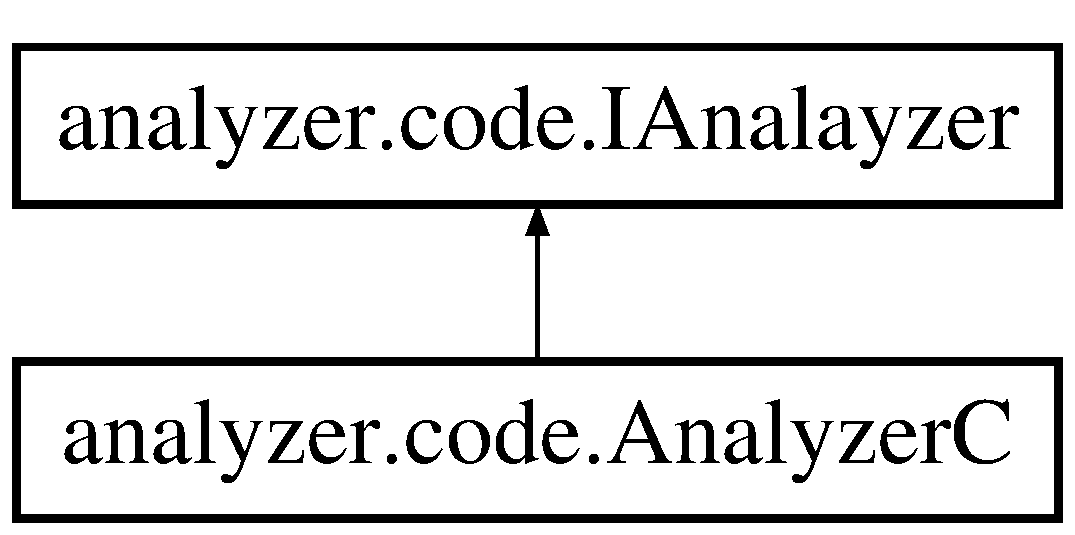
\includegraphics[height=2.000000cm]{classanalyzer_1_1code_1_1AnalyzerC}
\end{center}
\end{figure}
\subsection*{Public Member Functions}
\begin{DoxyCompactItemize}
\item 
\mbox{\Hypertarget{classanalyzer_1_1code_1_1AnalyzerC_a8740c2023bd7760c83abc8c630b5e121}\label{classanalyzer_1_1code_1_1AnalyzerC_a8740c2023bd7760c83abc8c630b5e121}} 
void {\bfseries solut\+Metrics} (String src)
\item 
\mbox{\Hypertarget{classanalyzer_1_1code_1_1AnalyzerC_a30bd977b7051d259f050445884486a31}\label{classanalyzer_1_1code_1_1AnalyzerC_a30bd977b7051d259f050445884486a31}} 
double {\bfseries get\+Mark} ()
\item 
\mbox{\Hypertarget{classanalyzer_1_1code_1_1AnalyzerC_ac96e4a7523afbcc244510bcfa8b39592}\label{classanalyzer_1_1code_1_1AnalyzerC_ac96e4a7523afbcc244510bcfa8b39592}} 
Array\+List$<$ List$<$ String $>$ $>$ {\bfseries get\+Result} ()
\item 
\mbox{\Hypertarget{classanalyzer_1_1code_1_1AnalyzerC_ada6b4b8177faa6d037226bdae4f827ce}\label{classanalyzer_1_1code_1_1AnalyzerC_ada6b4b8177faa6d037226bdae4f827ce}} 
void {\bfseries set\+Metric\+Settings} (Array\+List$<$ \hyperlink{classanalyzer_1_1code_1_1MetricSetting}{Metric\+Setting} $>$ metric\+Settings)
\item 
\mbox{\Hypertarget{classanalyzer_1_1code_1_1AnalyzerC_ae1858bb7eb088cd1bf0178e39af8f959}\label{classanalyzer_1_1code_1_1AnalyzerC_ae1858bb7eb088cd1bf0178e39af8f959}} 
void {\bfseries set\+Count\+Opetators\+Enable} (boolean enable)
\item 
\mbox{\Hypertarget{classanalyzer_1_1code_1_1AnalyzerC_a8d52368cccc22a8dff3f28d17afd1d5c}\label{classanalyzer_1_1code_1_1AnalyzerC_a8d52368cccc22a8dff3f28d17afd1d5c}} 
void {\bfseries setlevel\+Nest\+Enable} (boolean enable)
\item 
\mbox{\Hypertarget{classanalyzer_1_1code_1_1AnalyzerC_a466520117ab0a64f30798f0724c22dc2}\label{classanalyzer_1_1code_1_1AnalyzerC_a466520117ab0a64f30798f0724c22dc2}} 
void {\bfseries set\+Middle\+Len\+Ident\+Enable} (boolean enable)
\item 
\mbox{\Hypertarget{classanalyzer_1_1code_1_1AnalyzerC_a4cd5fd657befcff0c43b851ec503382c}\label{classanalyzer_1_1code_1_1AnalyzerC_a4cd5fd657befcff0c43b851ec503382c}} 
boolean {\bfseries is\+Count\+Operators\+Enable} ()
\item 
\mbox{\Hypertarget{classanalyzer_1_1code_1_1AnalyzerC_a69050bcc817ff2f824f69a5fd769f5b4}\label{classanalyzer_1_1code_1_1AnalyzerC_a69050bcc817ff2f824f69a5fd769f5b4}} 
boolean {\bfseries is\+Level\+Nest\+Enable} ()
\item 
\mbox{\Hypertarget{classanalyzer_1_1code_1_1AnalyzerC_a6ec503f9cbfb8f2525b85cfb10a86083}\label{classanalyzer_1_1code_1_1AnalyzerC_a6ec503f9cbfb8f2525b85cfb10a86083}} 
boolean {\bfseries is\+Middle\+Len\+Ident\+Enable} ()
\item 
\mbox{\Hypertarget{classanalyzer_1_1code_1_1AnalyzerC_a09e0bec3b91561d8f84e734d353ffbd4}\label{classanalyzer_1_1code_1_1AnalyzerC_a09e0bec3b91561d8f84e734d353ffbd4}} 
void {\bfseries set\+Level\+Nest\+Enable} (boolean level\+Nest\+Enable)
\item 
\mbox{\Hypertarget{classanalyzer_1_1code_1_1AnalyzerC_ac2f0d9485262b16d1f2910973a2124fe}\label{classanalyzer_1_1code_1_1AnalyzerC_ac2f0d9485262b16d1f2910973a2124fe}} 
double {\bfseries get\+Count\+Operator\+Project} ()
\item 
\mbox{\Hypertarget{classanalyzer_1_1code_1_1AnalyzerC_a3c0b693fe3c90fd7365fdca9331c3d2c}\label{classanalyzer_1_1code_1_1AnalyzerC_a3c0b693fe3c90fd7365fdca9331c3d2c}} 
double {\bfseries get\+Level\+Nest\+Project} ()
\item 
\mbox{\Hypertarget{classanalyzer_1_1code_1_1AnalyzerC_ac2d55c1faee58e2e891bda423d7762a4}\label{classanalyzer_1_1code_1_1AnalyzerC_ac2d55c1faee58e2e891bda423d7762a4}} 
double {\bfseries get\+Middle\+Len\+Ident\+Project} ()
\end{DoxyCompactItemize}


\subsection{Detailed Description}
\begin{DoxyAuthor}{Author}
tigler 
\end{DoxyAuthor}


The documentation for this class was generated from the following file\+:\begin{DoxyCompactItemize}
\item 
/home/tigler/\+Net\+Beans\+Projects/\+Plagiat/src/analyzer/code/Analyzer\+C.\+java\end{DoxyCompactItemize}

\hypertarget{classanalyzer_1_1code_1_1AnalyzerCode}{}\section{analyzer.\+code.\+Analyzer\+Code Class Reference}
\label{classanalyzer_1_1code_1_1AnalyzerCode}\index{analyzer.\+code.\+Analyzer\+Code@{analyzer.\+code.\+Analyzer\+Code}}
Inheritance diagram for analyzer.\+code.\+Analyzer\+Code\+:\begin{figure}[H]
\begin{center}
\leavevmode
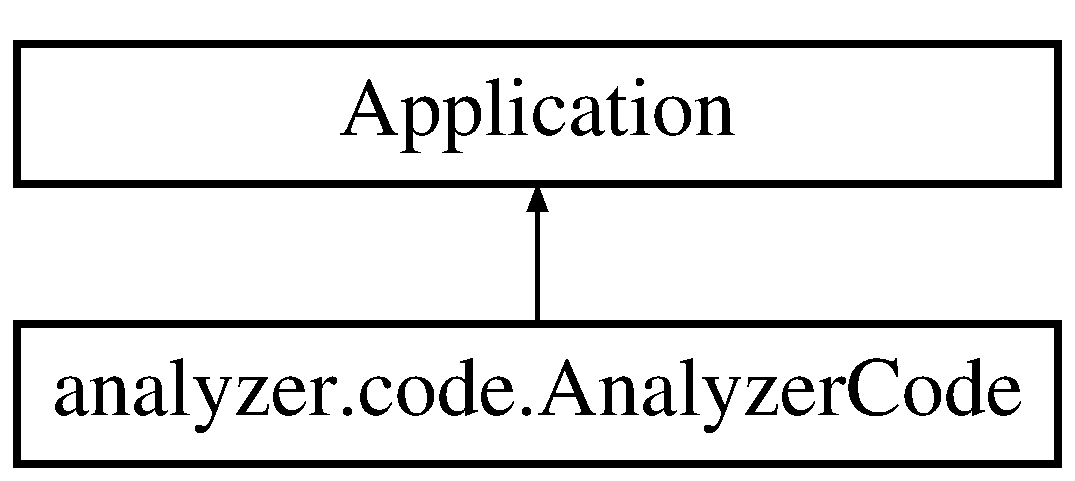
\includegraphics[height=2.000000cm]{classanalyzer_1_1code_1_1AnalyzerCode}
\end{center}
\end{figure}
\subsection*{Public Member Functions}
\begin{DoxyCompactItemize}
\item 
\mbox{\Hypertarget{classanalyzer_1_1code_1_1AnalyzerCode_ae7e73920c0e5911b5491f83325160fd7}\label{classanalyzer_1_1code_1_1AnalyzerCode_ae7e73920c0e5911b5491f83325160fd7}} 
void {\bfseries start} (Stage stage)  throws Exception 
\end{DoxyCompactItemize}
\subsection*{Static Public Member Functions}
\begin{DoxyCompactItemize}
\item 
static void \hyperlink{classanalyzer_1_1code_1_1AnalyzerCode_a60142285e91707f115ad27dccdf740eb}{main} (String\mbox{[}$\,$\mbox{]} args)
\end{DoxyCompactItemize}


\subsection{Detailed Description}
\begin{DoxyAuthor}{Author}
tigler 
\end{DoxyAuthor}


\subsection{Member Function Documentation}
\mbox{\Hypertarget{classanalyzer_1_1code_1_1AnalyzerCode_a60142285e91707f115ad27dccdf740eb}\label{classanalyzer_1_1code_1_1AnalyzerCode_a60142285e91707f115ad27dccdf740eb}} 
\index{analyzer\+::code\+::\+Analyzer\+Code@{analyzer\+::code\+::\+Analyzer\+Code}!main@{main}}
\index{main@{main}!analyzer\+::code\+::\+Analyzer\+Code@{analyzer\+::code\+::\+Analyzer\+Code}}
\subsubsection{\texorpdfstring{main()}{main()}}
{\footnotesize\ttfamily static void analyzer.\+code.\+Analyzer\+Code.\+main (\begin{DoxyParamCaption}\item[{String \mbox{[}$\,$\mbox{]}}]{args }\end{DoxyParamCaption})\hspace{0.3cm}{\ttfamily [inline]}, {\ttfamily [static]}}


\begin{DoxyParams}{Parameters}
{\em args} & the command line arguments \\
\hline
\end{DoxyParams}


The documentation for this class was generated from the following file\+:\begin{DoxyCompactItemize}
\item 
/home/tigler/\+Net\+Beans\+Projects/\+Plagiat/src/analyzer/code/Analyzer\+Code.\+java\end{DoxyCompactItemize}

\hypertarget{classanalyzer_1_1code_1_1CalculateMarkC}{}\section{analyzer.\+code.\+Calculate\+MarkC Class Reference}
\label{classanalyzer_1_1code_1_1CalculateMarkC}\index{analyzer.\+code.\+Calculate\+MarkC@{analyzer.\+code.\+Calculate\+MarkC}}
Inheritance diagram for analyzer.\+code.\+Calculate\+MarkC\+:\begin{figure}[H]
\begin{center}
\leavevmode
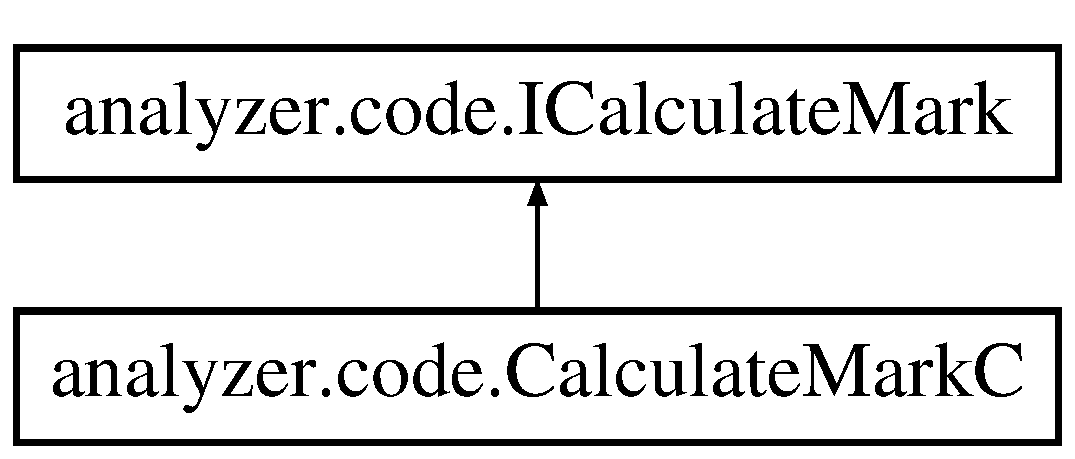
\includegraphics[height=2.000000cm]{classanalyzer_1_1code_1_1CalculateMarkC}
\end{center}
\end{figure}
\subsection*{Public Member Functions}
\begin{DoxyCompactItemize}
\item 
\mbox{\Hypertarget{classanalyzer_1_1code_1_1CalculateMarkC_ac94f8cd39b8581d49c98c0290a292ab7}\label{classanalyzer_1_1code_1_1CalculateMarkC_ac94f8cd39b8581d49c98c0290a292ab7}} 
double {\bfseries calcul\+Mark} (List$<$ Double $>$ metrs, Array\+List$<$ \hyperlink{classanalyzer_1_1code_1_1MetricSetting}{Metric\+Setting} $>$ metric\+Setting)
\end{DoxyCompactItemize}


\subsection{Detailed Description}
\begin{DoxyAuthor}{Author}
tigler 
\end{DoxyAuthor}


The documentation for this class was generated from the following file\+:\begin{DoxyCompactItemize}
\item 
/home/tigler/\+Net\+Beans\+Projects/\+Plagiat/src/analyzer/code/Calculate\+Mark\+C.\+java\end{DoxyCompactItemize}

\hypertarget{classanalyzer_1_1code_1_1CountOperators}{}\section{analyzer.\+code.\+Count\+Operators Class Reference}
\label{classanalyzer_1_1code_1_1CountOperators}\index{analyzer.\+code.\+Count\+Operators@{analyzer.\+code.\+Count\+Operators}}
Inheritance diagram for analyzer.\+code.\+Count\+Operators\+:\begin{figure}[H]
\begin{center}
\leavevmode
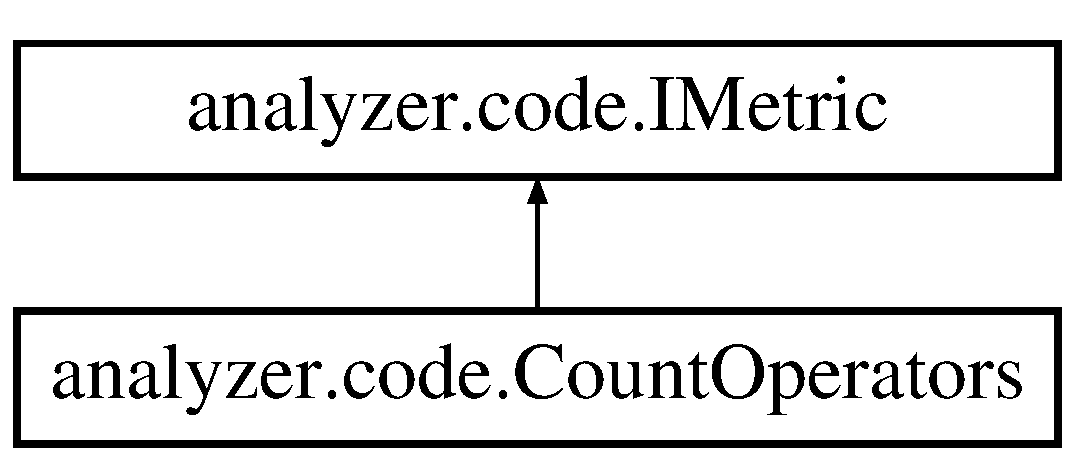
\includegraphics[height=2.000000cm]{classanalyzer_1_1code_1_1CountOperators}
\end{center}
\end{figure}
\subsection*{Public Member Functions}
\begin{DoxyCompactItemize}
\item 
\hyperlink{classanalyzer_1_1code_1_1CountOperators_a35cd40aef8c6e9b31aa51b667b7e3367}{Count\+Operators} ()
\item 
void \hyperlink{classanalyzer_1_1code_1_1CountOperators_a0dc10beb196cf80583707cbe4049eae2}{calculate} (\hyperlink{classanalyzer_1_1code_1_1Event}{Event} event)
\item 
double \hyperlink{classanalyzer_1_1code_1_1CountOperators_ab5d3d7000eaaa974536c967ceee9dcc7}{get\+Result} ()
\item 
void \hyperlink{classanalyzer_1_1code_1_1CountOperators_ad068949f06b712b55f12b03673a99278}{reset} ()
\end{DoxyCompactItemize}
\subsection*{Static Public Member Functions}
\begin{DoxyCompactItemize}
\item 
static String \hyperlink{classanalyzer_1_1code_1_1CountOperators_adce2eacc351b1a2c7d244a712d078477}{get\+Name} ()
\item 
static String \hyperlink{classanalyzer_1_1code_1_1CountOperators_aa89a8387e3c44af558eccf0733a98230}{get\+Mark} (double bad, double good, double metric)
\end{DoxyCompactItemize}


\subsection{Detailed Description}
Метрика просчета количества операторов между описанием и инициализацией переменной \begin{DoxyAuthor}{Author}
tigler 
\end{DoxyAuthor}


\subsection{Constructor \& Destructor Documentation}
\mbox{\Hypertarget{classanalyzer_1_1code_1_1CountOperators_a35cd40aef8c6e9b31aa51b667b7e3367}\label{classanalyzer_1_1code_1_1CountOperators_a35cd40aef8c6e9b31aa51b667b7e3367}} 
\index{analyzer\+::code\+::\+Count\+Operators@{analyzer\+::code\+::\+Count\+Operators}!Count\+Operators@{Count\+Operators}}
\index{Count\+Operators@{Count\+Operators}!analyzer\+::code\+::\+Count\+Operators@{analyzer\+::code\+::\+Count\+Operators}}
\subsubsection{\texorpdfstring{Count\+Operators()}{CountOperators()}}
{\footnotesize\ttfamily analyzer.\+code.\+Count\+Operators.\+Count\+Operators (\begin{DoxyParamCaption}{ }\end{DoxyParamCaption})\hspace{0.3cm}{\ttfamily [inline]}}

Конструктор без параметров -\/ инициализирует переменные класса\+: Array\+List$<$\+Variable$>$ variables, и int max\+Count\+Operator 

\subsection{Member Function Documentation}
\mbox{\Hypertarget{classanalyzer_1_1code_1_1CountOperators_a0dc10beb196cf80583707cbe4049eae2}\label{classanalyzer_1_1code_1_1CountOperators_a0dc10beb196cf80583707cbe4049eae2}} 
\index{analyzer\+::code\+::\+Count\+Operators@{analyzer\+::code\+::\+Count\+Operators}!calculate@{calculate}}
\index{calculate@{calculate}!analyzer\+::code\+::\+Count\+Operators@{analyzer\+::code\+::\+Count\+Operators}}
\subsubsection{\texorpdfstring{calculate()}{calculate()}}
{\footnotesize\ttfamily void analyzer.\+code.\+Count\+Operators.\+calculate (\begin{DoxyParamCaption}\item[{\hyperlink{classanalyzer_1_1code_1_1Event}{Event}}]{event }\end{DoxyParamCaption})\hspace{0.3cm}{\ttfamily [inline]}}

В зависимости от кода параметра event\+: Добавить переменную в список, если описание; Для каждой переменной инкрементировать их количество, если оператор; Вычислить максимальное количество операторов, если присваивание; Либо, не делать ничего. 
\begin{DoxyParams}{Parameters}
{\em event} & -\/ событие возникшее в синтаксическом анализаторе \\
\hline
\end{DoxyParams}


Implements \hyperlink{interfaceanalyzer_1_1code_1_1IMetric}{analyzer.\+code.\+I\+Metric}.

\mbox{\Hypertarget{classanalyzer_1_1code_1_1CountOperators_aa89a8387e3c44af558eccf0733a98230}\label{classanalyzer_1_1code_1_1CountOperators_aa89a8387e3c44af558eccf0733a98230}} 
\index{analyzer\+::code\+::\+Count\+Operators@{analyzer\+::code\+::\+Count\+Operators}!get\+Mark@{get\+Mark}}
\index{get\+Mark@{get\+Mark}!analyzer\+::code\+::\+Count\+Operators@{analyzer\+::code\+::\+Count\+Operators}}
\subsubsection{\texorpdfstring{get\+Mark()}{getMark()}}
{\footnotesize\ttfamily static String analyzer.\+code.\+Count\+Operators.\+get\+Mark (\begin{DoxyParamCaption}\item[{double}]{bad,  }\item[{double}]{good,  }\item[{double}]{metric }\end{DoxyParamCaption})\hspace{0.3cm}{\ttfamily [inline]}, {\ttfamily [static]}}

Статический метод для получения описания оценки.


\begin{DoxyParams}{Parameters}
{\em bad} & -\/ значение плохой оценки \\
\hline
{\em good} & -\/ значение хорошей оценки \\
\hline
{\em metric} & -\/ текущая оценка \\
\hline
\end{DoxyParams}
\begin{DoxyReturn}{Returns}
Строку оценки, в зависимости от значений параметров 
\end{DoxyReturn}
\mbox{\Hypertarget{classanalyzer_1_1code_1_1CountOperators_adce2eacc351b1a2c7d244a712d078477}\label{classanalyzer_1_1code_1_1CountOperators_adce2eacc351b1a2c7d244a712d078477}} 
\index{analyzer\+::code\+::\+Count\+Operators@{analyzer\+::code\+::\+Count\+Operators}!get\+Name@{get\+Name}}
\index{get\+Name@{get\+Name}!analyzer\+::code\+::\+Count\+Operators@{analyzer\+::code\+::\+Count\+Operators}}
\subsubsection{\texorpdfstring{get\+Name()}{getName()}}
{\footnotesize\ttfamily static String analyzer.\+code.\+Count\+Operators.\+get\+Name (\begin{DoxyParamCaption}{ }\end{DoxyParamCaption})\hspace{0.3cm}{\ttfamily [inline]}, {\ttfamily [static]}}

Статический метод для получения названия метрики. Использует перечисление \hyperlink{enumanalyzer_1_1code_1_1EnumNamesMetric}{Enum\+Names\+Metric} с названиями метрик. \begin{DoxyReturn}{Returns}
Строку -\/ навание метрики. 
\end{DoxyReturn}
\mbox{\Hypertarget{classanalyzer_1_1code_1_1CountOperators_ab5d3d7000eaaa974536c967ceee9dcc7}\label{classanalyzer_1_1code_1_1CountOperators_ab5d3d7000eaaa974536c967ceee9dcc7}} 
\index{analyzer\+::code\+::\+Count\+Operators@{analyzer\+::code\+::\+Count\+Operators}!get\+Result@{get\+Result}}
\index{get\+Result@{get\+Result}!analyzer\+::code\+::\+Count\+Operators@{analyzer\+::code\+::\+Count\+Operators}}
\subsubsection{\texorpdfstring{get\+Result()}{getResult()}}
{\footnotesize\ttfamily double analyzer.\+code.\+Count\+Operators.\+get\+Result (\begin{DoxyParamCaption}{ }\end{DoxyParamCaption})\hspace{0.3cm}{\ttfamily [inline]}}

Получить максимальное количество операторов между описанием и присваиванием \begin{DoxyReturn}{Returns}
переменную max\+Count\+Operator 
\end{DoxyReturn}


Implements \hyperlink{interfaceanalyzer_1_1code_1_1IMetric}{analyzer.\+code.\+I\+Metric}.

\mbox{\Hypertarget{classanalyzer_1_1code_1_1CountOperators_ad068949f06b712b55f12b03673a99278}\label{classanalyzer_1_1code_1_1CountOperators_ad068949f06b712b55f12b03673a99278}} 
\index{analyzer\+::code\+::\+Count\+Operators@{analyzer\+::code\+::\+Count\+Operators}!reset@{reset}}
\index{reset@{reset}!analyzer\+::code\+::\+Count\+Operators@{analyzer\+::code\+::\+Count\+Operators}}
\subsubsection{\texorpdfstring{reset()}{reset()}}
{\footnotesize\ttfamily void analyzer.\+code.\+Count\+Operators.\+reset (\begin{DoxyParamCaption}{ }\end{DoxyParamCaption})\hspace{0.3cm}{\ttfamily [inline]}}

cбрасывает значения переменных до начальных 

Implements \hyperlink{interfaceanalyzer_1_1code_1_1IMetric}{analyzer.\+code.\+I\+Metric}.



The documentation for this class was generated from the following file\+:\begin{DoxyCompactItemize}
\item 
/home/tigler/\+Net\+Beans\+Projects/\+Plagiat/src/analyzer/code/Count\+Operators.\+java\end{DoxyCompactItemize}

\hypertarget{enumanalyzer_1_1code_1_1EnumMarkCountOperators}{}\section{analyzer.\+code.\+Enum\+Mark\+Count\+Operators Enum Reference}
\label{enumanalyzer_1_1code_1_1EnumMarkCountOperators}\index{analyzer.\+code.\+Enum\+Mark\+Count\+Operators@{analyzer.\+code.\+Enum\+Mark\+Count\+Operators}}
\subsection*{Public Member Functions}
\begin{DoxyCompactItemize}
\item 
\mbox{\Hypertarget{enumanalyzer_1_1code_1_1EnumMarkCountOperators_aa561144f51585ce5b6aa8900688baf15}\label{enumanalyzer_1_1code_1_1EnumMarkCountOperators_aa561144f51585ce5b6aa8900688baf15}} 
String {\bfseries to\+String} ()
\end{DoxyCompactItemize}
\subsection*{Public Attributes}
\begin{DoxyCompactItemize}
\item 
\mbox{\Hypertarget{enumanalyzer_1_1code_1_1EnumMarkCountOperators_acc5d0b694750267c0779663fbb88371e}\label{enumanalyzer_1_1code_1_1EnumMarkCountOperators_acc5d0b694750267c0779663fbb88371e}} 
{\bfseries mode1} =(\char`\"{}Много операторов между\textbackslash{}nописанием и присваиванием.\textbackslash{}nИнициализацию нужно\textbackslash{}nпроводить раньше.\char`\"{})
\item 
\mbox{\Hypertarget{enumanalyzer_1_1code_1_1EnumMarkCountOperators_a2ee4665764352e78a8124eb3969bcba4}\label{enumanalyzer_1_1code_1_1EnumMarkCountOperators_a2ee4665764352e78a8124eb3969bcba4}} 
{\bfseries mode2} =(\char`\"{}Количество операторов\textbackslash{}nмежду описанием и\textbackslash{}nприсваиванием в норме\char`\"{})
\item 
\mbox{\Hypertarget{enumanalyzer_1_1code_1_1EnumMarkCountOperators_abad4ece73bc89def2c2c07a8bae1d030}\label{enumanalyzer_1_1code_1_1EnumMarkCountOperators_abad4ece73bc89def2c2c07a8bae1d030}} 
{\bfseries mode3} =(\char`\"{}Kоличество операторов\textbackslash{}nмежду описанием и\textbackslash{}nприсваиванием соответвтвует\textbackslash{}nкачественному коду\char`\"{})
\end{DoxyCompactItemize}


\subsection{Detailed Description}
\begin{DoxyAuthor}{Author}
tigler 
\end{DoxyAuthor}


The documentation for this enum was generated from the following file\+:\begin{DoxyCompactItemize}
\item 
/home/tigler/\+Net\+Beans\+Projects/\+Plagiat/src/analyzer/code/Enum\+Mark\+Count\+Operators.\+java\end{DoxyCompactItemize}

\hypertarget{enumanalyzer_1_1code_1_1EnumMarkLevelNest}{}\section{analyzer.\+code.\+Enum\+Mark\+Level\+Nest Enum Reference}
\label{enumanalyzer_1_1code_1_1EnumMarkLevelNest}\index{analyzer.\+code.\+Enum\+Mark\+Level\+Nest@{analyzer.\+code.\+Enum\+Mark\+Level\+Nest}}
\subsection*{Public Member Functions}
\begin{DoxyCompactItemize}
\item 
String \hyperlink{enumanalyzer_1_1code_1_1EnumMarkLevelNest_a00997fede2fe10301bff2b5a023685d3}{to\+String} ()
\end{DoxyCompactItemize}
\subsection*{Public Attributes}
\begin{DoxyCompactItemize}
\item 
\mbox{\Hypertarget{enumanalyzer_1_1code_1_1EnumMarkLevelNest_a5ac19926bb8f5e3673869c621695c5d8}\label{enumanalyzer_1_1code_1_1EnumMarkLevelNest_a5ac19926bb8f5e3673869c621695c5d8}} 
{\bfseries mode1} =(\char`\"{}Уровень вложенности\textbackslash{}nоператоров if большой.\char`\"{})
\item 
\mbox{\Hypertarget{enumanalyzer_1_1code_1_1EnumMarkLevelNest_a0727d5b6ba587aebe1f1cfd70c9a0e32}\label{enumanalyzer_1_1code_1_1EnumMarkLevelNest_a0727d5b6ba587aebe1f1cfd70c9a0e32}} 
{\bfseries mode2} =(\char`\"{}Уровень вложенности\textbackslash{}nоператоров if в норме\char`\"{})
\item 
\mbox{\Hypertarget{enumanalyzer_1_1code_1_1EnumMarkLevelNest_a9dbfbf7b32361b97ced37b90df5ad631}\label{enumanalyzer_1_1code_1_1EnumMarkLevelNest_a9dbfbf7b32361b97ced37b90df5ad631}} 
{\bfseries mode3} =(\char`\"{}Уровень вложенности\textbackslash{}nоператоров if\textbackslash{}nсоответвтвует\textbackslash{}nкачественному коду\char`\"{})
\end{DoxyCompactItemize}


\subsection{Detailed Description}
Перечисление оценок для метрики \char`\"{}Максимальный уровень вложенности if\char`\"{} \begin{DoxyAuthor}{Author}
tigler 
\end{DoxyAuthor}


\subsection{Member Function Documentation}
\mbox{\Hypertarget{enumanalyzer_1_1code_1_1EnumMarkLevelNest_a00997fede2fe10301bff2b5a023685d3}\label{enumanalyzer_1_1code_1_1EnumMarkLevelNest_a00997fede2fe10301bff2b5a023685d3}} 
\index{analyzer\+::code\+::\+Enum\+Mark\+Level\+Nest@{analyzer\+::code\+::\+Enum\+Mark\+Level\+Nest}!to\+String@{to\+String}}
\index{to\+String@{to\+String}!analyzer\+::code\+::\+Enum\+Mark\+Level\+Nest@{analyzer\+::code\+::\+Enum\+Mark\+Level\+Nest}}
\subsubsection{\texorpdfstring{to\+String()}{toString()}}
{\footnotesize\ttfamily String analyzer.\+code.\+Enum\+Mark\+Level\+Nest.\+to\+String (\begin{DoxyParamCaption}{ }\end{DoxyParamCaption})\hspace{0.3cm}{\ttfamily [inline]}}

Получить строку с оценкой. \begin{DoxyReturn}{Returns}
Строку с оценкой. 
\end{DoxyReturn}


The documentation for this enum was generated from the following file\+:\begin{DoxyCompactItemize}
\item 
/home/tigler/\+Net\+Beans\+Projects/\+Plagiat/src/analyzer/code/Enum\+Mark\+Level\+Nest.\+java\end{DoxyCompactItemize}

\hypertarget{enumanalyzer_1_1code_1_1EnumMarkMiddleLenIdent}{}\section{analyzer.\+code.\+Enum\+Mark\+Middle\+Len\+Ident Enum Reference}
\label{enumanalyzer_1_1code_1_1EnumMarkMiddleLenIdent}\index{analyzer.\+code.\+Enum\+Mark\+Middle\+Len\+Ident@{analyzer.\+code.\+Enum\+Mark\+Middle\+Len\+Ident}}
\subsection*{Public Member Functions}
\begin{DoxyCompactItemize}
\item 
String \hyperlink{enumanalyzer_1_1code_1_1EnumMarkMiddleLenIdent_a057938ee5095c35298a6c7741f7d0cb3}{to\+String} ()
\end{DoxyCompactItemize}
\subsection*{Public Attributes}
\begin{DoxyCompactItemize}
\item 
\mbox{\Hypertarget{enumanalyzer_1_1code_1_1EnumMarkMiddleLenIdent_ae226ba41e31793d6073db62e639d1b6a}\label{enumanalyzer_1_1code_1_1EnumMarkMiddleLenIdent_ae226ba41e31793d6073db62e639d1b6a}} 
{\bfseries mode1} =(\char`\"{}Длина идентификатора\textbackslash{}nслишком мала.\textbackslash{}nКод не читаемый\char`\"{})
\item 
\mbox{\Hypertarget{enumanalyzer_1_1code_1_1EnumMarkMiddleLenIdent_a9f139e7a82637b8fe23235af49a17d9f}\label{enumanalyzer_1_1code_1_1EnumMarkMiddleLenIdent_a9f139e7a82637b8fe23235af49a17d9f}} 
{\bfseries mode2} =(\char`\"{}Длина идентификаторов\textbackslash{}nв норме.\textbackslash{}nКод читаемый\char`\"{})
\item 
\mbox{\Hypertarget{enumanalyzer_1_1code_1_1EnumMarkMiddleLenIdent_a10054d78e462584beeb4666b2de03bb9}\label{enumanalyzer_1_1code_1_1EnumMarkMiddleLenIdent_a10054d78e462584beeb4666b2de03bb9}} 
{\bfseries mode3} =(\char`\"{}Длина идентификаторов\textbackslash{}nслишком велика\textbackslash{}nсоздается нагромождение\char`\"{})
\end{DoxyCompactItemize}


\subsection{Detailed Description}
Перечисление оценок для метрики \char`\"{}Средняя длина идентификатора\char`\"{} \begin{DoxyAuthor}{Author}
tigler 
\end{DoxyAuthor}


\subsection{Member Function Documentation}
\mbox{\Hypertarget{enumanalyzer_1_1code_1_1EnumMarkMiddleLenIdent_a057938ee5095c35298a6c7741f7d0cb3}\label{enumanalyzer_1_1code_1_1EnumMarkMiddleLenIdent_a057938ee5095c35298a6c7741f7d0cb3}} 
\index{analyzer\+::code\+::\+Enum\+Mark\+Middle\+Len\+Ident@{analyzer\+::code\+::\+Enum\+Mark\+Middle\+Len\+Ident}!to\+String@{to\+String}}
\index{to\+String@{to\+String}!analyzer\+::code\+::\+Enum\+Mark\+Middle\+Len\+Ident@{analyzer\+::code\+::\+Enum\+Mark\+Middle\+Len\+Ident}}
\subsubsection{\texorpdfstring{to\+String()}{toString()}}
{\footnotesize\ttfamily String analyzer.\+code.\+Enum\+Mark\+Middle\+Len\+Ident.\+to\+String (\begin{DoxyParamCaption}{ }\end{DoxyParamCaption})\hspace{0.3cm}{\ttfamily [inline]}}

Получить строку с оценкой. \begin{DoxyReturn}{Returns}
Строку с оценкой. 
\end{DoxyReturn}


The documentation for this enum was generated from the following file\+:\begin{DoxyCompactItemize}
\item 
/home/tigler/\+Net\+Beans\+Projects/\+Plagiat/src/analyzer/code/Enum\+Mark\+Middle\+Len\+Ident.\+java\end{DoxyCompactItemize}

\hypertarget{enumanalyzer_1_1code_1_1EnumNameMetricC}{}\section{analyzer.\+code.\+Enum\+Name\+MetricC Enum Reference}
\label{enumanalyzer_1_1code_1_1EnumNameMetricC}\index{analyzer.\+code.\+Enum\+Name\+MetricC@{analyzer.\+code.\+Enum\+Name\+MetricC}}
\subsection*{Public Member Functions}
\begin{DoxyCompactItemize}
\item 
String \hyperlink{enumanalyzer_1_1code_1_1EnumNameMetricC_a4520d230bcc68d57f67d1bd2f6d009ba}{get\+Name} ()
\end{DoxyCompactItemize}
\subsection*{Public Attributes}
\begin{DoxyCompactItemize}
\item 
\mbox{\Hypertarget{enumanalyzer_1_1code_1_1EnumNameMetricC_a093c21844bf187b178956b737b633f06}\label{enumanalyzer_1_1code_1_1EnumNameMetricC_a093c21844bf187b178956b737b633f06}} 
{\bfseries mode1} =(\char`\"{}Count\+Operators\char`\"{})
\item 
\mbox{\Hypertarget{enumanalyzer_1_1code_1_1EnumNameMetricC_a96288f32ed1267f33360f0d4a0c1cd72}\label{enumanalyzer_1_1code_1_1EnumNameMetricC_a96288f32ed1267f33360f0d4a0c1cd72}} 
{\bfseries mode2} =(\char`\"{}Level Nest\char`\"{})
\item 
\mbox{\Hypertarget{enumanalyzer_1_1code_1_1EnumNameMetricC_a3cd74e4e95ea10304281ec3d86c07c10}\label{enumanalyzer_1_1code_1_1EnumNameMetricC_a3cd74e4e95ea10304281ec3d86c07c10}} 
{\bfseries mode3} =(\char`\"{}Middle Len Ident\char`\"{})
\end{DoxyCompactItemize}


\subsection{Detailed Description}
Перечисление наименований метрик языка С. \begin{DoxyAuthor}{Author}
tigler 
\end{DoxyAuthor}


\subsection{Member Function Documentation}
\mbox{\Hypertarget{enumanalyzer_1_1code_1_1EnumNameMetricC_a4520d230bcc68d57f67d1bd2f6d009ba}\label{enumanalyzer_1_1code_1_1EnumNameMetricC_a4520d230bcc68d57f67d1bd2f6d009ba}} 
\index{analyzer\+::code\+::\+Enum\+Name\+MetricC@{analyzer\+::code\+::\+Enum\+Name\+MetricC}!get\+Name@{get\+Name}}
\index{get\+Name@{get\+Name}!analyzer\+::code\+::\+Enum\+Name\+MetricC@{analyzer\+::code\+::\+Enum\+Name\+MetricC}}
\subsubsection{\texorpdfstring{get\+Name()}{getName()}}
{\footnotesize\ttfamily String analyzer.\+code.\+Enum\+Name\+Metric\+C.\+get\+Name (\begin{DoxyParamCaption}{ }\end{DoxyParamCaption})\hspace{0.3cm}{\ttfamily [inline]}}

Получить название метрики. \begin{DoxyReturn}{Returns}
Строку-\/ название метрики. 
\end{DoxyReturn}


The documentation for this enum was generated from the following file\+:\begin{DoxyCompactItemize}
\item 
/home/tigler/\+Net\+Beans\+Projects/\+Plagiat/src/analyzer/code/Enum\+Name\+Metric\+C.\+java\end{DoxyCompactItemize}

\hypertarget{enumanalyzer_1_1code_1_1EnumNamesMetric}{}\section{analyzer.\+code.\+Enum\+Names\+Metric Enum Reference}
\label{enumanalyzer_1_1code_1_1EnumNamesMetric}\index{analyzer.\+code.\+Enum\+Names\+Metric@{analyzer.\+code.\+Enum\+Names\+Metric}}
\subsection*{Public Member Functions}
\begin{DoxyCompactItemize}
\item 
String \hyperlink{enumanalyzer_1_1code_1_1EnumNamesMetric_a3ddc0d95ae5e93f08fa6273ea4c308a7}{to\+String} ()
\end{DoxyCompactItemize}
\subsection*{Public Attributes}
\begin{DoxyCompactItemize}
\item 
\mbox{\Hypertarget{enumanalyzer_1_1code_1_1EnumNamesMetric_a492e123ac37a4cfcc15c7ac62be6faed}\label{enumanalyzer_1_1code_1_1EnumNamesMetric_a492e123ac37a4cfcc15c7ac62be6faed}} 
{\bfseries mode1} =(\char`\"{}Count\+Operators\char`\"{})
\item 
\mbox{\Hypertarget{enumanalyzer_1_1code_1_1EnumNamesMetric_a8a20b91930a031b90ce4c002e1304243}\label{enumanalyzer_1_1code_1_1EnumNamesMetric_a8a20b91930a031b90ce4c002e1304243}} 
{\bfseries mode2} =(\char`\"{}Level Nest\char`\"{})
\item 
\mbox{\Hypertarget{enumanalyzer_1_1code_1_1EnumNamesMetric_ab414c78a055b8758e2998a7f5c38dd57}\label{enumanalyzer_1_1code_1_1EnumNamesMetric_ab414c78a055b8758e2998a7f5c38dd57}} 
{\bfseries mode3} =(\char`\"{}Middle Len Ident\char`\"{})
\end{DoxyCompactItemize}


\subsection{Detailed Description}
Перечисление наименований метрик языка. \begin{DoxyAuthor}{Author}
tigler 
\end{DoxyAuthor}


\subsection{Member Function Documentation}
\mbox{\Hypertarget{enumanalyzer_1_1code_1_1EnumNamesMetric_a3ddc0d95ae5e93f08fa6273ea4c308a7}\label{enumanalyzer_1_1code_1_1EnumNamesMetric_a3ddc0d95ae5e93f08fa6273ea4c308a7}} 
\index{analyzer\+::code\+::\+Enum\+Names\+Metric@{analyzer\+::code\+::\+Enum\+Names\+Metric}!to\+String@{to\+String}}
\index{to\+String@{to\+String}!analyzer\+::code\+::\+Enum\+Names\+Metric@{analyzer\+::code\+::\+Enum\+Names\+Metric}}
\subsubsection{\texorpdfstring{to\+String()}{toString()}}
{\footnotesize\ttfamily String analyzer.\+code.\+Enum\+Names\+Metric.\+to\+String (\begin{DoxyParamCaption}{ }\end{DoxyParamCaption})\hspace{0.3cm}{\ttfamily [inline]}}

Получить название метрики. \begin{DoxyReturn}{Returns}
Строку-\/ название метрики. 
\end{DoxyReturn}


The documentation for this enum was generated from the following file\+:\begin{DoxyCompactItemize}
\item 
/home/tigler/\+Net\+Beans\+Projects/\+Plagiat/src/analyzer/code/Enum\+Names\+Metric.\+java\end{DoxyCompactItemize}

\hypertarget{classanalyzer_1_1code_1_1Event}{}\section{analyzer.\+code.\+Event Class Reference}
\label{classanalyzer_1_1code_1_1Event}\index{analyzer.\+code.\+Event@{analyzer.\+code.\+Event}}


\subsection{Detailed Description}
Событие происходящее в синтаксическом анализаторе. Типы событий\+: начало if, конец if, описание переменной, присваивание, оператор, индентификатор. \begin{DoxyAuthor}{Author}
tigler 
\end{DoxyAuthor}


The documentation for this class was generated from the following file\+:\begin{DoxyCompactItemize}
\item 
/home/tigler/\+Net\+Beans\+Projects/\+Plagiat/src/analyzer/code/Event.\+java\end{DoxyCompactItemize}

\hypertarget{classanalyzer_1_1code_1_1EventCountOperator}{}\section{analyzer.\+code.\+Event\+Count\+Operator Class Reference}
\label{classanalyzer_1_1code_1_1EventCountOperator}\index{analyzer.\+code.\+Event\+Count\+Operator@{analyzer.\+code.\+Event\+Count\+Operator}}
Inheritance diagram for analyzer.\+code.\+Event\+Count\+Operator\+:\begin{figure}[H]
\begin{center}
\leavevmode
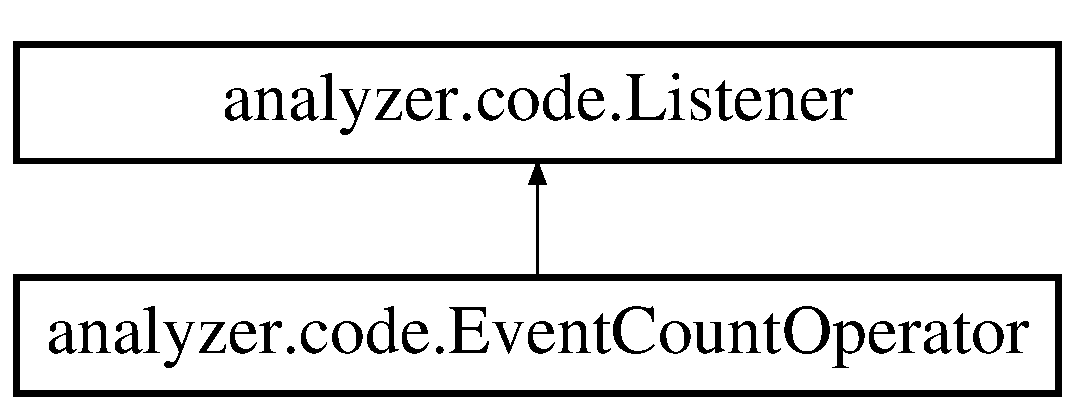
\includegraphics[height=2.000000cm]{classanalyzer_1_1code_1_1EventCountOperator}
\end{center}
\end{figure}
\subsection*{Public Member Functions}
\begin{DoxyCompactItemize}
\item 
\mbox{\Hypertarget{classanalyzer_1_1code_1_1EventCountOperator_a74ef4c2d87ce6b3ff05194e74893e8c4}\label{classanalyzer_1_1code_1_1EventCountOperator_a74ef4c2d87ce6b3ff05194e74893e8c4}} 
{\bfseries Event\+Count\+Operator} (\hyperlink{interfaceanalyzer_1_1code_1_1IMetric}{I\+Metric} ce)
\item 
\mbox{\Hypertarget{classanalyzer_1_1code_1_1EventCountOperator_ac8a9f1fafedc773a304a5949b948e960}\label{classanalyzer_1_1code_1_1EventCountOperator_ac8a9f1fafedc773a304a5949b948e960}} 
{\bfseries Event\+Count\+Operator} (\hyperlink{interfaceanalyzer_1_1code_1_1IMetric}{I\+Metric} ce, \hyperlink{classanalyzer_1_1code_1_1Listener}{Listener} successer)
\item 
\mbox{\Hypertarget{classanalyzer_1_1code_1_1EventCountOperator_abd2a8d557f0cae911e61133c0e90697b}\label{classanalyzer_1_1code_1_1EventCountOperator_abd2a8d557f0cae911e61133c0e90697b}} 
void {\bfseries on\+Event} (\hyperlink{classanalyzer_1_1code_1_1Event}{Event} event)
\end{DoxyCompactItemize}


\subsection{Detailed Description}
\begin{DoxyAuthor}{Author}
tigler 
\end{DoxyAuthor}


The documentation for this class was generated from the following file\+:\begin{DoxyCompactItemize}
\item 
/home/tigler/\+Net\+Beans\+Projects/\+Plagiat/src/analyzer/code/Event\+Count\+Operator.\+java\end{DoxyCompactItemize}

\hypertarget{classanalyzer_1_1code_1_1EventLevelNest}{}\section{analyzer.\+code.\+Event\+Level\+Nest Class Reference}
\label{classanalyzer_1_1code_1_1EventLevelNest}\index{analyzer.\+code.\+Event\+Level\+Nest@{analyzer.\+code.\+Event\+Level\+Nest}}
Inheritance diagram for analyzer.\+code.\+Event\+Level\+Nest\+:\begin{figure}[H]
\begin{center}
\leavevmode
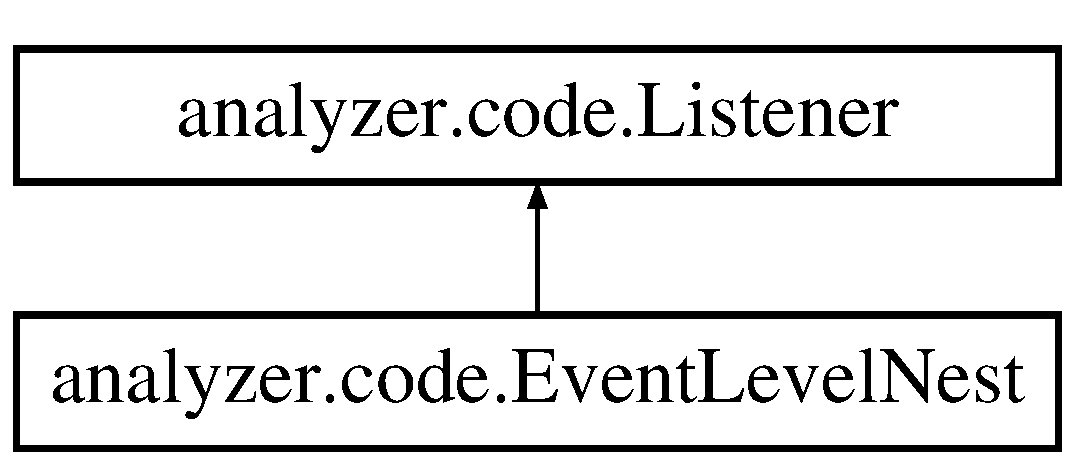
\includegraphics[height=2.000000cm]{classanalyzer_1_1code_1_1EventLevelNest}
\end{center}
\end{figure}
\subsection*{Public Member Functions}
\begin{DoxyCompactItemize}
\item 
\mbox{\Hypertarget{classanalyzer_1_1code_1_1EventLevelNest_a9958fcecfabb6bde976c193145089c04}\label{classanalyzer_1_1code_1_1EventLevelNest_a9958fcecfabb6bde976c193145089c04}} 
{\bfseries Event\+Level\+Nest} (\hyperlink{interfaceanalyzer_1_1code_1_1IMetric}{I\+Metric} ln)
\item 
\mbox{\Hypertarget{classanalyzer_1_1code_1_1EventLevelNest_a4544f1e67e498e0d913aaf1b663a4d3c}\label{classanalyzer_1_1code_1_1EventLevelNest_a4544f1e67e498e0d913aaf1b663a4d3c}} 
{\bfseries Event\+Level\+Nest} (\hyperlink{interfaceanalyzer_1_1code_1_1IMetric}{I\+Metric} ln, \hyperlink{classanalyzer_1_1code_1_1Listener}{Listener} successor)
\item 
\mbox{\Hypertarget{classanalyzer_1_1code_1_1EventLevelNest_a4f22be2013be45803dbb7fb3f5f06c7b}\label{classanalyzer_1_1code_1_1EventLevelNest_a4f22be2013be45803dbb7fb3f5f06c7b}} 
void {\bfseries on\+Event} (\hyperlink{classanalyzer_1_1code_1_1Event}{Event} event)
\end{DoxyCompactItemize}


\subsection{Detailed Description}
\begin{DoxyAuthor}{Author}
tigler 
\end{DoxyAuthor}


The documentation for this class was generated from the following file\+:\begin{DoxyCompactItemize}
\item 
/home/tigler/\+Net\+Beans\+Projects/\+Plagiat/src/analyzer/code/Event\+Level\+Nest.\+java\end{DoxyCompactItemize}

\hypertarget{classanalyzer_1_1code_1_1EventMiddleLenIdent}{}\section{analyzer.\+code.\+Event\+Middle\+Len\+Ident Class Reference}
\label{classanalyzer_1_1code_1_1EventMiddleLenIdent}\index{analyzer.\+code.\+Event\+Middle\+Len\+Ident@{analyzer.\+code.\+Event\+Middle\+Len\+Ident}}
Inheritance diagram for analyzer.\+code.\+Event\+Middle\+Len\+Ident\+:\begin{figure}[H]
\begin{center}
\leavevmode
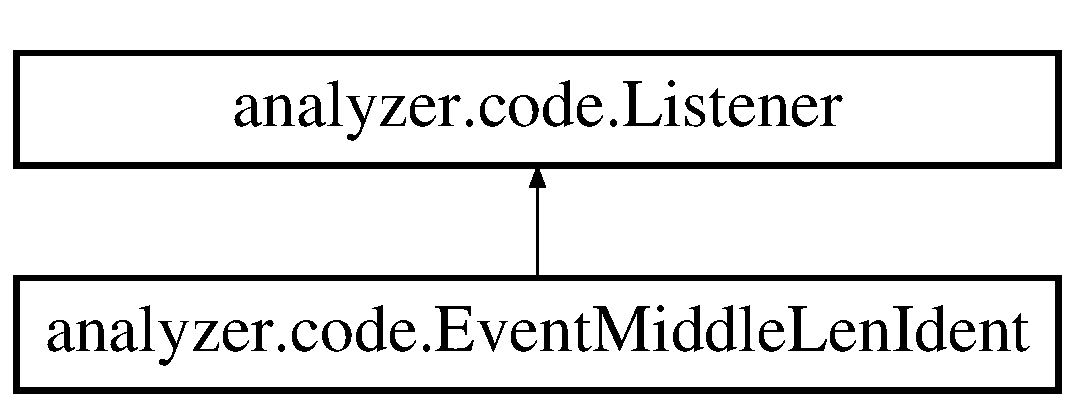
\includegraphics[height=2.000000cm]{classanalyzer_1_1code_1_1EventMiddleLenIdent}
\end{center}
\end{figure}
\subsection*{Public Member Functions}
\begin{DoxyCompactItemize}
\item 
\mbox{\Hypertarget{classanalyzer_1_1code_1_1EventMiddleLenIdent_a995a9b0ac22753aa10ca5abebca442dc}\label{classanalyzer_1_1code_1_1EventMiddleLenIdent_a995a9b0ac22753aa10ca5abebca442dc}} 
{\bfseries Event\+Middle\+Len\+Ident} (\hyperlink{interfaceanalyzer_1_1code_1_1IMetric}{I\+Metric} mli)
\item 
\mbox{\Hypertarget{classanalyzer_1_1code_1_1EventMiddleLenIdent_a3f84d2a99cdee3688fef3c42cb613bbc}\label{classanalyzer_1_1code_1_1EventMiddleLenIdent_a3f84d2a99cdee3688fef3c42cb613bbc}} 
{\bfseries Event\+Middle\+Len\+Ident} (\hyperlink{interfaceanalyzer_1_1code_1_1IMetric}{I\+Metric} mli, \hyperlink{classanalyzer_1_1code_1_1Listener}{Listener} succsessor)
\item 
\mbox{\Hypertarget{classanalyzer_1_1code_1_1EventMiddleLenIdent_ad5c28b67f1dac29d4cbda885cb54ce92}\label{classanalyzer_1_1code_1_1EventMiddleLenIdent_ad5c28b67f1dac29d4cbda885cb54ce92}} 
void {\bfseries on\+Event} (\hyperlink{classanalyzer_1_1code_1_1Event}{Event} event)
\end{DoxyCompactItemize}


\subsection{Detailed Description}
\begin{DoxyAuthor}{Author}
tigler 
\end{DoxyAuthor}


The documentation for this class was generated from the following file\+:\begin{DoxyCompactItemize}
\item 
/home/tigler/\+Net\+Beans\+Projects/\+Plagiat/src/analyzer/code/Event\+Middle\+Len\+Ident.\+java\end{DoxyCompactItemize}

\hypertarget{classanalyzer_1_1code_1_1FXMLAboutProgrammController}{}\section{analyzer.\+code.\+F\+X\+M\+L\+About\+Programm\+Controller Class Reference}
\label{classanalyzer_1_1code_1_1FXMLAboutProgrammController}\index{analyzer.\+code.\+F\+X\+M\+L\+About\+Programm\+Controller@{analyzer.\+code.\+F\+X\+M\+L\+About\+Programm\+Controller}}
Inheritance diagram for analyzer.\+code.\+F\+X\+M\+L\+About\+Programm\+Controller\+:\begin{figure}[H]
\begin{center}
\leavevmode
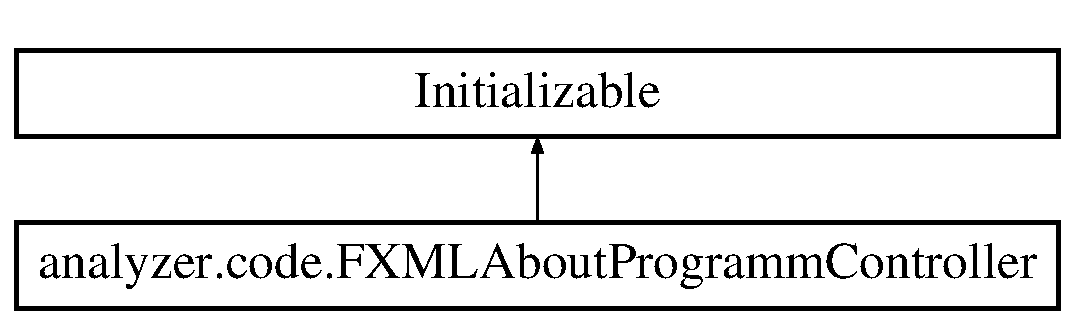
\includegraphics[height=2.000000cm]{classanalyzer_1_1code_1_1FXMLAboutProgrammController}
\end{center}
\end{figure}
\subsection*{Public Member Functions}
\begin{DoxyCompactItemize}
\item 
void \hyperlink{classanalyzer_1_1code_1_1FXMLAboutProgrammController_aa4aaf33b2bb1bb10d95af39c294dbec8}{initialize} (U\+RL url, Resource\+Bundle rb)
\end{DoxyCompactItemize}


\subsection{Detailed Description}
F\+X\+ML Controller class

\begin{DoxyAuthor}{Author}
tigler 
\end{DoxyAuthor}


\subsection{Member Function Documentation}
\mbox{\Hypertarget{classanalyzer_1_1code_1_1FXMLAboutProgrammController_aa4aaf33b2bb1bb10d95af39c294dbec8}\label{classanalyzer_1_1code_1_1FXMLAboutProgrammController_aa4aaf33b2bb1bb10d95af39c294dbec8}} 
\index{analyzer\+::code\+::\+F\+X\+M\+L\+About\+Programm\+Controller@{analyzer\+::code\+::\+F\+X\+M\+L\+About\+Programm\+Controller}!initialize@{initialize}}
\index{initialize@{initialize}!analyzer\+::code\+::\+F\+X\+M\+L\+About\+Programm\+Controller@{analyzer\+::code\+::\+F\+X\+M\+L\+About\+Programm\+Controller}}
\subsubsection{\texorpdfstring{initialize()}{initialize()}}
{\footnotesize\ttfamily void analyzer.\+code.\+F\+X\+M\+L\+About\+Programm\+Controller.\+initialize (\begin{DoxyParamCaption}\item[{U\+RL}]{url,  }\item[{Resource\+Bundle}]{rb }\end{DoxyParamCaption})\hspace{0.3cm}{\ttfamily [inline]}}

Initializes the controller class. 

The documentation for this class was generated from the following file\+:\begin{DoxyCompactItemize}
\item 
/home/tigler/\+Net\+Beans\+Projects/\+Plagiat/src/analyzer/code/F\+X\+M\+L\+About\+Programm\+Controller.\+java\end{DoxyCompactItemize}

\hypertarget{classanalyzer_1_1code_1_1FXMLAnalyzerController}{}\section{analyzer.\+code.\+F\+X\+M\+L\+Analyzer\+Controller Class Reference}
\label{classanalyzer_1_1code_1_1FXMLAnalyzerController}\index{analyzer.\+code.\+F\+X\+M\+L\+Analyzer\+Controller@{analyzer.\+code.\+F\+X\+M\+L\+Analyzer\+Controller}}
Inheritance diagram for analyzer.\+code.\+F\+X\+M\+L\+Analyzer\+Controller\+:\begin{figure}[H]
\begin{center}
\leavevmode
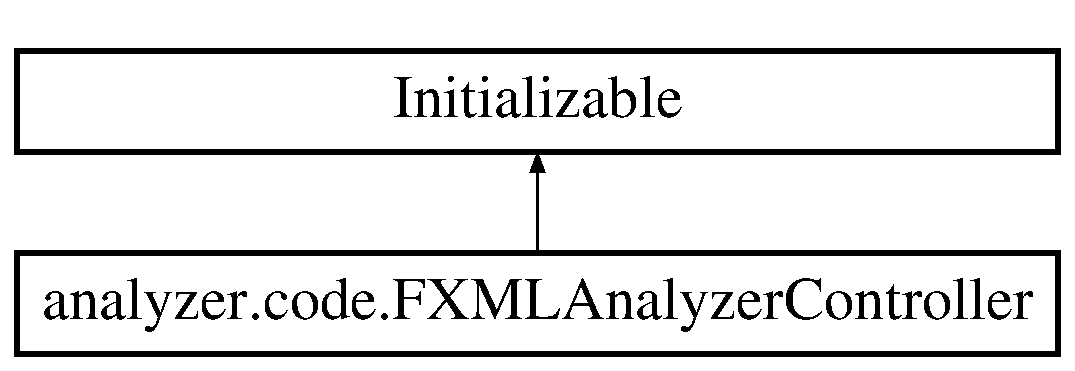
\includegraphics[height=2.000000cm]{classanalyzer_1_1code_1_1FXMLAnalyzerController}
\end{center}
\end{figure}
\subsection*{Public Member Functions}
\begin{DoxyCompactItemize}
\item 
\mbox{\Hypertarget{classanalyzer_1_1code_1_1FXMLAnalyzerController_a742d7b4fb9f500ccba85a7e6e60c8283}\label{classanalyzer_1_1code_1_1FXMLAnalyzerController_a742d7b4fb9f500ccba85a7e6e60c8283}} 
Array\+List$<$ Array\+List$<$ \hyperlink{classanalyzer_1_1code_1_1MetricSetting}{Metric\+Setting} $>$ $>$ {\bfseries get\+Metric\+Settings} ()
\item 
\mbox{\Hypertarget{classanalyzer_1_1code_1_1FXMLAnalyzerController_aaae0681946ade2af2356aa45c2ed202f}\label{classanalyzer_1_1code_1_1FXMLAnalyzerController_aaae0681946ade2af2356aa45c2ed202f}} 
Array\+List$<$ Array\+List$<$ \hyperlink{classanalyzer_1_1code_1_1MetricSetting}{Metric\+Setting} $>$ $>$ {\bfseries get\+Metric\+Settings\+Def} ()
\item 
\mbox{\Hypertarget{classanalyzer_1_1code_1_1FXMLAnalyzerController_a2cd9499872c25effdb902574f2f484b7}\label{classanalyzer_1_1code_1_1FXMLAnalyzerController_a2cd9499872c25effdb902574f2f484b7}} 
void {\bfseries initialize} (U\+RL url, Resource\+Bundle rb)
\end{DoxyCompactItemize}


\subsection{Detailed Description}
\begin{DoxyAuthor}{Author}
tigler 
\end{DoxyAuthor}


The documentation for this class was generated from the following file\+:\begin{DoxyCompactItemize}
\item 
/home/tigler/\+Net\+Beans\+Projects/\+Plagiat/src/analyzer/code/F\+X\+M\+L\+Analyzer\+Controller.\+java\end{DoxyCompactItemize}

\hypertarget{classanalyzer_1_1code_1_1FXMLMetricsController}{}\section{analyzer.\+code.\+F\+X\+M\+L\+Metrics\+Controller Class Reference}
\label{classanalyzer_1_1code_1_1FXMLMetricsController}\index{analyzer.\+code.\+F\+X\+M\+L\+Metrics\+Controller@{analyzer.\+code.\+F\+X\+M\+L\+Metrics\+Controller}}
Inheritance diagram for analyzer.\+code.\+F\+X\+M\+L\+Metrics\+Controller\+:\begin{figure}[H]
\begin{center}
\leavevmode
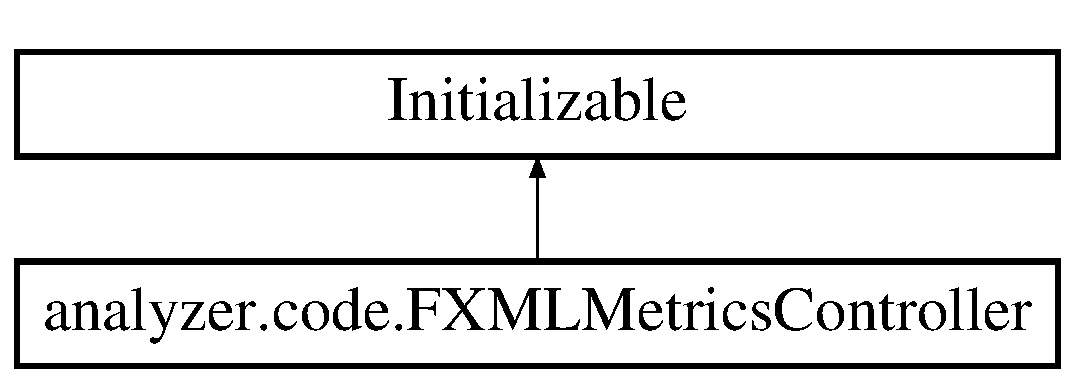
\includegraphics[height=2.000000cm]{classanalyzer_1_1code_1_1FXMLMetricsController}
\end{center}
\end{figure}
\subsection*{Public Member Functions}
\begin{DoxyCompactItemize}
\item 
\mbox{\Hypertarget{classanalyzer_1_1code_1_1FXMLMetricsController_a2d7edaf36849da79f67532a3dc789d18}\label{classanalyzer_1_1code_1_1FXMLMetricsController_a2d7edaf36849da79f67532a3dc789d18}} 
void {\bfseries set\+Analyzer} (\hyperlink{classanalyzer_1_1code_1_1AnalyzerC}{AnalyzerC} analayzer)
\item 
void \hyperlink{classanalyzer_1_1code_1_1FXMLMetricsController_ae7fea4d81f2544c571d453a61f24e845}{initialize} (U\+RL url, Resource\+Bundle rb)
\end{DoxyCompactItemize}


\subsection{Detailed Description}
F\+X\+ML Controller class

\begin{DoxyAuthor}{Author}
tigler 
\end{DoxyAuthor}


\subsection{Member Function Documentation}
\mbox{\Hypertarget{classanalyzer_1_1code_1_1FXMLMetricsController_ae7fea4d81f2544c571d453a61f24e845}\label{classanalyzer_1_1code_1_1FXMLMetricsController_ae7fea4d81f2544c571d453a61f24e845}} 
\index{analyzer\+::code\+::\+F\+X\+M\+L\+Metrics\+Controller@{analyzer\+::code\+::\+F\+X\+M\+L\+Metrics\+Controller}!initialize@{initialize}}
\index{initialize@{initialize}!analyzer\+::code\+::\+F\+X\+M\+L\+Metrics\+Controller@{analyzer\+::code\+::\+F\+X\+M\+L\+Metrics\+Controller}}
\subsubsection{\texorpdfstring{initialize()}{initialize()}}
{\footnotesize\ttfamily void analyzer.\+code.\+F\+X\+M\+L\+Metrics\+Controller.\+initialize (\begin{DoxyParamCaption}\item[{U\+RL}]{url,  }\item[{Resource\+Bundle}]{rb }\end{DoxyParamCaption})\hspace{0.3cm}{\ttfamily [inline]}}

Initializes the controller class. 

The documentation for this class was generated from the following file\+:\begin{DoxyCompactItemize}
\item 
/home/tigler/\+Net\+Beans\+Projects/\+Plagiat/src/analyzer/code/F\+X\+M\+L\+Metrics\+Controller.\+java\end{DoxyCompactItemize}

\hypertarget{classanalyzer_1_1code_1_1FXMLSelectUsedProjectController}{}\section{analyzer.\+code.\+F\+X\+M\+L\+Select\+Used\+Project\+Controller Class Reference}
\label{classanalyzer_1_1code_1_1FXMLSelectUsedProjectController}\index{analyzer.\+code.\+F\+X\+M\+L\+Select\+Used\+Project\+Controller@{analyzer.\+code.\+F\+X\+M\+L\+Select\+Used\+Project\+Controller}}
Inheritance diagram for analyzer.\+code.\+F\+X\+M\+L\+Select\+Used\+Project\+Controller\+:\begin{figure}[H]
\begin{center}
\leavevmode
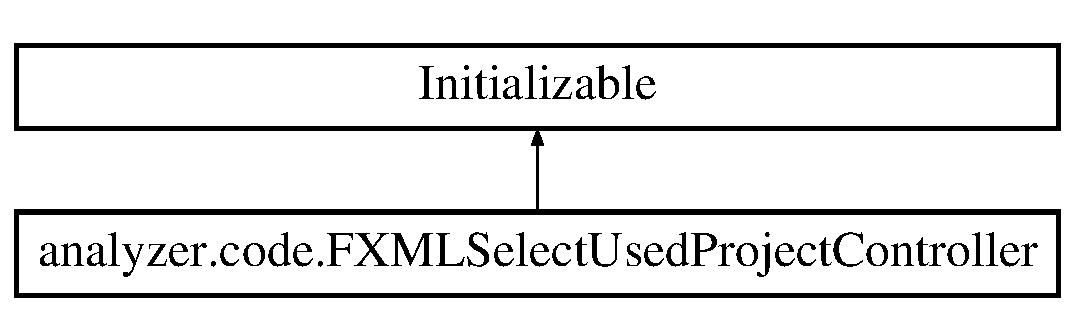
\includegraphics[height=2.000000cm]{classanalyzer_1_1code_1_1FXMLSelectUsedProjectController}
\end{center}
\end{figure}
\subsection*{Public Member Functions}
\begin{DoxyCompactItemize}
\item 
void \hyperlink{classanalyzer_1_1code_1_1FXMLSelectUsedProjectController_afe6580b67e899e3bb10ffc60713ec005}{initialize} (U\+RL url, Resource\+Bundle rb)
\end{DoxyCompactItemize}


\subsection{Detailed Description}
F\+X\+ML Controller class

\begin{DoxyAuthor}{Author}
tigler 
\end{DoxyAuthor}


\subsection{Member Function Documentation}
\mbox{\Hypertarget{classanalyzer_1_1code_1_1FXMLSelectUsedProjectController_afe6580b67e899e3bb10ffc60713ec005}\label{classanalyzer_1_1code_1_1FXMLSelectUsedProjectController_afe6580b67e899e3bb10ffc60713ec005}} 
\index{analyzer\+::code\+::\+F\+X\+M\+L\+Select\+Used\+Project\+Controller@{analyzer\+::code\+::\+F\+X\+M\+L\+Select\+Used\+Project\+Controller}!initialize@{initialize}}
\index{initialize@{initialize}!analyzer\+::code\+::\+F\+X\+M\+L\+Select\+Used\+Project\+Controller@{analyzer\+::code\+::\+F\+X\+M\+L\+Select\+Used\+Project\+Controller}}
\subsubsection{\texorpdfstring{initialize()}{initialize()}}
{\footnotesize\ttfamily void analyzer.\+code.\+F\+X\+M\+L\+Select\+Used\+Project\+Controller.\+initialize (\begin{DoxyParamCaption}\item[{U\+RL}]{url,  }\item[{Resource\+Bundle}]{rb }\end{DoxyParamCaption})\hspace{0.3cm}{\ttfamily [inline]}}

Initializes the controller class. 

The documentation for this class was generated from the following file\+:\begin{DoxyCompactItemize}
\item 
/home/tigler/\+Net\+Beans\+Projects/\+Plagiat/src/analyzer/code/F\+X\+M\+L\+Select\+Used\+Project\+Controller.\+java\end{DoxyCompactItemize}

\hypertarget{classanalyzer_1_1code_1_1FXMLSettingController}{}\section{analyzer.\+code.\+F\+X\+M\+L\+Setting\+Controller Class Reference}
\label{classanalyzer_1_1code_1_1FXMLSettingController}\index{analyzer.\+code.\+F\+X\+M\+L\+Setting\+Controller@{analyzer.\+code.\+F\+X\+M\+L\+Setting\+Controller}}
Inheritance diagram for analyzer.\+code.\+F\+X\+M\+L\+Setting\+Controller\+:\begin{figure}[H]
\begin{center}
\leavevmode
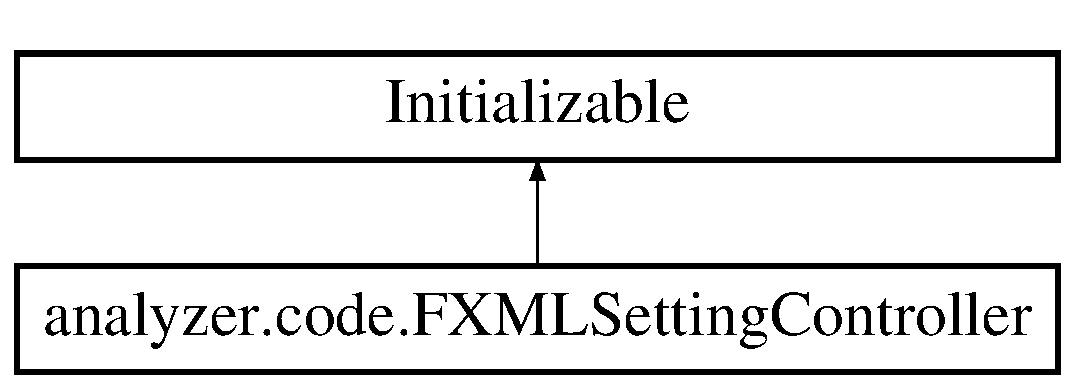
\includegraphics[height=2.000000cm]{classanalyzer_1_1code_1_1FXMLSettingController}
\end{center}
\end{figure}
\subsection*{Public Member Functions}
\begin{DoxyCompactItemize}
\item 
void \hyperlink{classanalyzer_1_1code_1_1FXMLSettingController_acaccf0fd8287b68a3845acbbe31efe95}{initialize} (U\+RL url, Resource\+Bundle rb)
\end{DoxyCompactItemize}


\subsection{Detailed Description}
F\+X\+ML Controller class

\begin{DoxyAuthor}{Author}
tigler 
\end{DoxyAuthor}


\subsection{Member Function Documentation}
\mbox{\Hypertarget{classanalyzer_1_1code_1_1FXMLSettingController_acaccf0fd8287b68a3845acbbe31efe95}\label{classanalyzer_1_1code_1_1FXMLSettingController_acaccf0fd8287b68a3845acbbe31efe95}} 
\index{analyzer\+::code\+::\+F\+X\+M\+L\+Setting\+Controller@{analyzer\+::code\+::\+F\+X\+M\+L\+Setting\+Controller}!initialize@{initialize}}
\index{initialize@{initialize}!analyzer\+::code\+::\+F\+X\+M\+L\+Setting\+Controller@{analyzer\+::code\+::\+F\+X\+M\+L\+Setting\+Controller}}
\subsubsection{\texorpdfstring{initialize()}{initialize()}}
{\footnotesize\ttfamily void analyzer.\+code.\+F\+X\+M\+L\+Setting\+Controller.\+initialize (\begin{DoxyParamCaption}\item[{U\+RL}]{url,  }\item[{Resource\+Bundle}]{rb }\end{DoxyParamCaption})\hspace{0.3cm}{\ttfamily [inline]}}

Initializes the controller class. 

The documentation for this class was generated from the following file\+:\begin{DoxyCompactItemize}
\item 
/home/tigler/\+Net\+Beans\+Projects/\+Plagiat/src/analyzer/code/F\+X\+M\+L\+Setting\+Controller.\+java\end{DoxyCompactItemize}

\hypertarget{interfaceanalyzer_1_1code_1_1IAnalayzer}{}\section{analyzer.\+code.\+I\+Analayzer Interface Reference}
\label{interfaceanalyzer_1_1code_1_1IAnalayzer}\index{analyzer.\+code.\+I\+Analayzer@{analyzer.\+code.\+I\+Analayzer}}
Inheritance diagram for analyzer.\+code.\+I\+Analayzer\+:\begin{figure}[H]
\begin{center}
\leavevmode
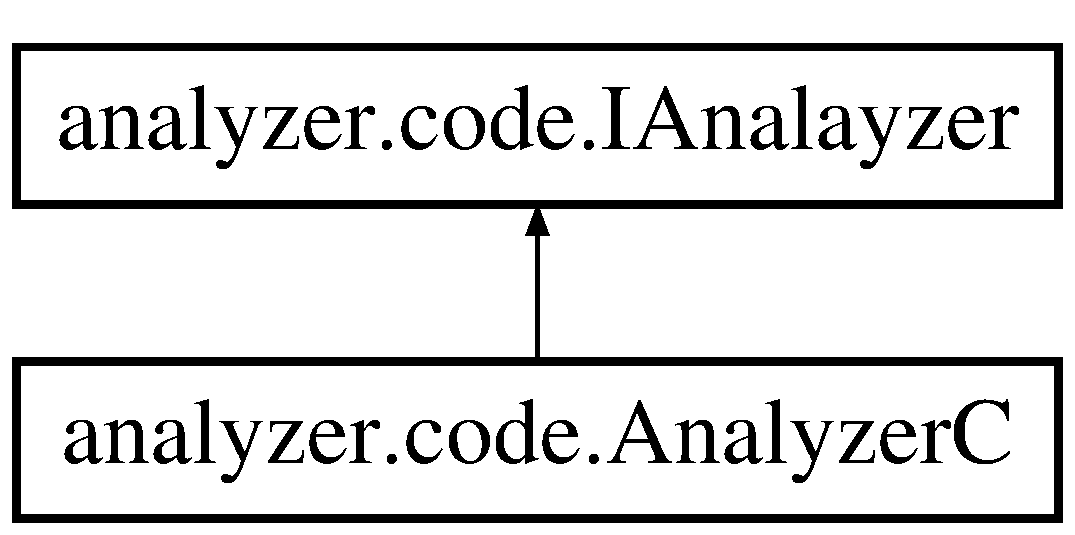
\includegraphics[height=2.000000cm]{interfaceanalyzer_1_1code_1_1IAnalayzer}
\end{center}
\end{figure}
\subsection*{Public Member Functions}
\begin{DoxyCompactItemize}
\item 
\mbox{\Hypertarget{interfaceanalyzer_1_1code_1_1IAnalayzer_a450ba935983e53a70454ab92a0981cc2}\label{interfaceanalyzer_1_1code_1_1IAnalayzer_a450ba935983e53a70454ab92a0981cc2}} 
void {\bfseries solut\+Metrics} (String src)
\item 
\mbox{\Hypertarget{interfaceanalyzer_1_1code_1_1IAnalayzer_add27d4f396a1cf411f44dc8cf151f89a}\label{interfaceanalyzer_1_1code_1_1IAnalayzer_add27d4f396a1cf411f44dc8cf151f89a}} 
double {\bfseries get\+Mark} ()
\item 
\mbox{\Hypertarget{interfaceanalyzer_1_1code_1_1IAnalayzer_a3a30c70be99d63443660aa5a6180ef8e}\label{interfaceanalyzer_1_1code_1_1IAnalayzer_a3a30c70be99d63443660aa5a6180ef8e}} 
Array\+List$<$ List$<$ String $>$ $>$ {\bfseries get\+Result} ()
\item 
\mbox{\Hypertarget{interfaceanalyzer_1_1code_1_1IAnalayzer_a2940a978e68d01c8a66d3dcf213b577a}\label{interfaceanalyzer_1_1code_1_1IAnalayzer_a2940a978e68d01c8a66d3dcf213b577a}} 
void {\bfseries set\+Metric\+Settings} (Array\+List$<$ \hyperlink{classanalyzer_1_1code_1_1MetricSetting}{Metric\+Setting} $>$ metric\+Settings)
\end{DoxyCompactItemize}


\subsection{Detailed Description}
\begin{DoxyAuthor}{Author}
tigler 
\end{DoxyAuthor}


The documentation for this interface was generated from the following file\+:\begin{DoxyCompactItemize}
\item 
/home/tigler/\+Net\+Beans\+Projects/\+Plagiat/src/analyzer/code/I\+Analayzer.\+java\end{DoxyCompactItemize}

\hypertarget{interfaceanalyzer_1_1code_1_1ICalculateMark}{}\section{analyzer.\+code.\+I\+Calculate\+Mark Interface Reference}
\label{interfaceanalyzer_1_1code_1_1ICalculateMark}\index{analyzer.\+code.\+I\+Calculate\+Mark@{analyzer.\+code.\+I\+Calculate\+Mark}}
Inheritance diagram for analyzer.\+code.\+I\+Calculate\+Mark\+:\begin{figure}[H]
\begin{center}
\leavevmode
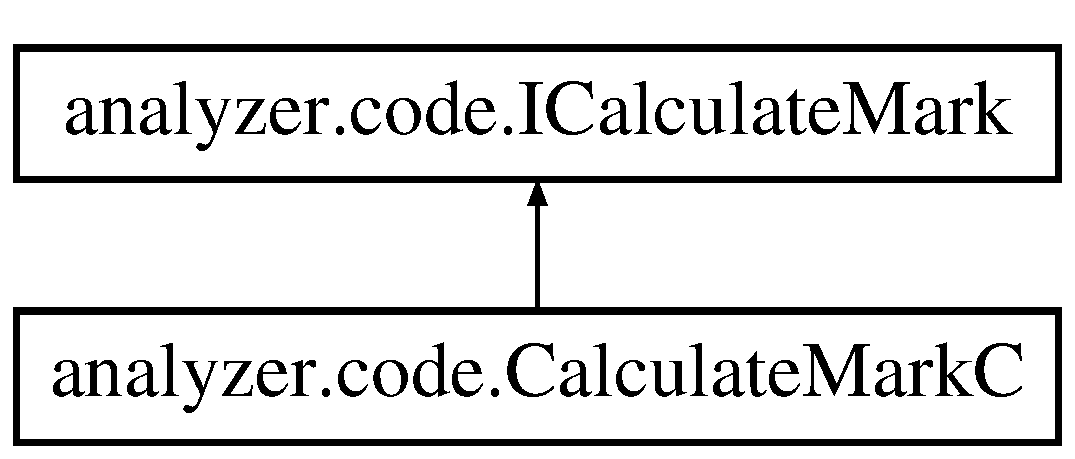
\includegraphics[height=2.000000cm]{interfaceanalyzer_1_1code_1_1ICalculateMark}
\end{center}
\end{figure}
\subsection*{Public Member Functions}
\begin{DoxyCompactItemize}
\item 
\mbox{\Hypertarget{interfaceanalyzer_1_1code_1_1ICalculateMark_ad1e7a2d4fcffa56b451910cc521ce7f4}\label{interfaceanalyzer_1_1code_1_1ICalculateMark_ad1e7a2d4fcffa56b451910cc521ce7f4}} 
double {\bfseries calcul\+Mark} (List$<$ Double $>$ metrs, Array\+List$<$ \hyperlink{classanalyzer_1_1code_1_1MetricSetting}{Metric\+Setting} $>$ metric\+Setting)
\end{DoxyCompactItemize}


\subsection{Detailed Description}
\begin{DoxyAuthor}{Author}
tigler 
\end{DoxyAuthor}


The documentation for this interface was generated from the following file\+:\begin{DoxyCompactItemize}
\item 
/home/tigler/\+Net\+Beans\+Projects/\+Plagiat/src/analyzer/code/I\+Calculate\+Mark.\+java\end{DoxyCompactItemize}

\hypertarget{interfaceanalyzer_1_1code_1_1IMetric}{}\section{analyzer.\+code.\+I\+Metric Interface Reference}
\label{interfaceanalyzer_1_1code_1_1IMetric}\index{analyzer.\+code.\+I\+Metric@{analyzer.\+code.\+I\+Metric}}
Inheritance diagram for analyzer.\+code.\+I\+Metric\+:\begin{figure}[H]
\begin{center}
\leavevmode
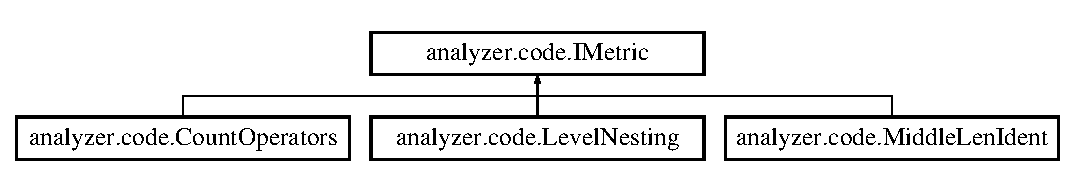
\includegraphics[height=1.914530cm]{interfaceanalyzer_1_1code_1_1IMetric}
\end{center}
\end{figure}
\subsection*{Public Member Functions}
\begin{DoxyCompactItemize}
\item 
\mbox{\Hypertarget{interfaceanalyzer_1_1code_1_1IMetric_af282cdf9099b9c71af2b3ba1ef678d39}\label{interfaceanalyzer_1_1code_1_1IMetric_af282cdf9099b9c71af2b3ba1ef678d39}} 
void {\bfseries calculate} (\hyperlink{classanalyzer_1_1code_1_1Event}{Event} event)
\item 
\mbox{\Hypertarget{interfaceanalyzer_1_1code_1_1IMetric_a86779b844f595f60a13e51946c57b4db}\label{interfaceanalyzer_1_1code_1_1IMetric_a86779b844f595f60a13e51946c57b4db}} 
void {\bfseries reset} ()
\item 
\mbox{\Hypertarget{interfaceanalyzer_1_1code_1_1IMetric_a43d08f765fbc75476186d2d3a576fe99}\label{interfaceanalyzer_1_1code_1_1IMetric_a43d08f765fbc75476186d2d3a576fe99}} 
double {\bfseries get\+Result} ()
\end{DoxyCompactItemize}


\subsection{Detailed Description}
\begin{DoxyAuthor}{Author}
tigler 
\end{DoxyAuthor}


The documentation for this interface was generated from the following file\+:\begin{DoxyCompactItemize}
\item 
/home/tigler/\+Net\+Beans\+Projects/\+Plagiat/src/analyzer/code/I\+Metric.\+java\end{DoxyCompactItemize}

\hypertarget{classanalyzer_1_1code_1_1LevelNesting}{}\section{analyzer.\+code.\+Level\+Nesting Class Reference}
\label{classanalyzer_1_1code_1_1LevelNesting}\index{analyzer.\+code.\+Level\+Nesting@{analyzer.\+code.\+Level\+Nesting}}
Inheritance diagram for analyzer.\+code.\+Level\+Nesting\+:\begin{figure}[H]
\begin{center}
\leavevmode
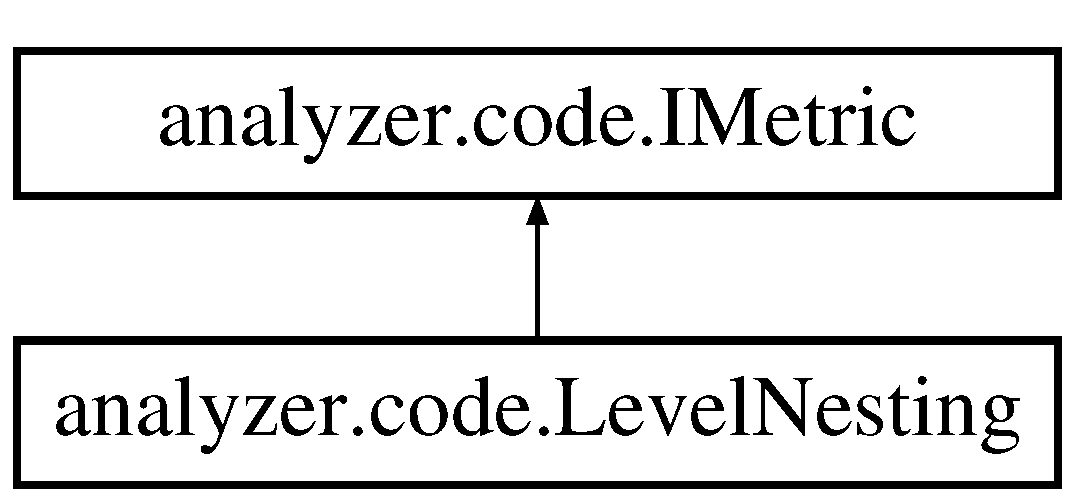
\includegraphics[height=2.000000cm]{classanalyzer_1_1code_1_1LevelNesting}
\end{center}
\end{figure}
\subsection*{Public Member Functions}
\begin{DoxyCompactItemize}
\item 
\hyperlink{classanalyzer_1_1code_1_1LevelNesting_ae2b01629780a540f7e261ce2c59d654e}{Level\+Nesting} ()
\item 
void \hyperlink{classanalyzer_1_1code_1_1LevelNesting_a09431a19031d65f2e53257c9d10beb49}{calculate} (\hyperlink{classanalyzer_1_1code_1_1Event}{Event} event)
\item 
double \hyperlink{classanalyzer_1_1code_1_1LevelNesting_ab16151c8d69cb40a84d73b2a9574fd85}{get\+Result} ()
\item 
void \hyperlink{classanalyzer_1_1code_1_1LevelNesting_a5aeb52565e529607aa8a3b2bd4beb490}{reset} ()
\end{DoxyCompactItemize}
\subsection*{Static Public Member Functions}
\begin{DoxyCompactItemize}
\item 
static String \hyperlink{classanalyzer_1_1code_1_1LevelNesting_aea9db3974d2a58fb0b559c830a0386c1}{get\+Name} ()
\item 
static String \hyperlink{classanalyzer_1_1code_1_1LevelNesting_a6e56b6f52fc6eb7b5645ce24e5dfe370}{get\+Mark} (double bad, double good, double metric)
\end{DoxyCompactItemize}


\subsection{Detailed Description}
Определяет максимальный уровень вложенности оператара if \begin{DoxyAuthor}{Author}
tigler 
\end{DoxyAuthor}


\subsection{Constructor \& Destructor Documentation}
\mbox{\Hypertarget{classanalyzer_1_1code_1_1LevelNesting_ae2b01629780a540f7e261ce2c59d654e}\label{classanalyzer_1_1code_1_1LevelNesting_ae2b01629780a540f7e261ce2c59d654e}} 
\index{analyzer\+::code\+::\+Level\+Nesting@{analyzer\+::code\+::\+Level\+Nesting}!Level\+Nesting@{Level\+Nesting}}
\index{Level\+Nesting@{Level\+Nesting}!analyzer\+::code\+::\+Level\+Nesting@{analyzer\+::code\+::\+Level\+Nesting}}
\subsubsection{\texorpdfstring{Level\+Nesting()}{LevelNesting()}}
{\footnotesize\ttfamily analyzer.\+code.\+Level\+Nesting.\+Level\+Nesting (\begin{DoxyParamCaption}{ }\end{DoxyParamCaption})\hspace{0.3cm}{\ttfamily [inline]}}

Конструктор без параметров, инициализирует переменные экзмепляра. 

\subsection{Member Function Documentation}
\mbox{\Hypertarget{classanalyzer_1_1code_1_1LevelNesting_a09431a19031d65f2e53257c9d10beb49}\label{classanalyzer_1_1code_1_1LevelNesting_a09431a19031d65f2e53257c9d10beb49}} 
\index{analyzer\+::code\+::\+Level\+Nesting@{analyzer\+::code\+::\+Level\+Nesting}!calculate@{calculate}}
\index{calculate@{calculate}!analyzer\+::code\+::\+Level\+Nesting@{analyzer\+::code\+::\+Level\+Nesting}}
\subsubsection{\texorpdfstring{calculate()}{calculate()}}
{\footnotesize\ttfamily void analyzer.\+code.\+Level\+Nesting.\+calculate (\begin{DoxyParamCaption}\item[{\hyperlink{classanalyzer_1_1code_1_1Event}{Event}}]{event }\end{DoxyParamCaption})\hspace{0.3cm}{\ttfamily [inline]}}

В зависимости от кода параметра event, изменяет максимальный, и текущий уровень вложенности. 
\begin{DoxyParams}{Parameters}
{\em event} & -\/ -\/ событие возникшее в синтаксическом анализаторе \\
\hline
\end{DoxyParams}


Implements \hyperlink{interfaceanalyzer_1_1code_1_1IMetric}{analyzer.\+code.\+I\+Metric}.

\mbox{\Hypertarget{classanalyzer_1_1code_1_1LevelNesting_a6e56b6f52fc6eb7b5645ce24e5dfe370}\label{classanalyzer_1_1code_1_1LevelNesting_a6e56b6f52fc6eb7b5645ce24e5dfe370}} 
\index{analyzer\+::code\+::\+Level\+Nesting@{analyzer\+::code\+::\+Level\+Nesting}!get\+Mark@{get\+Mark}}
\index{get\+Mark@{get\+Mark}!analyzer\+::code\+::\+Level\+Nesting@{analyzer\+::code\+::\+Level\+Nesting}}
\subsubsection{\texorpdfstring{get\+Mark()}{getMark()}}
{\footnotesize\ttfamily static String analyzer.\+code.\+Level\+Nesting.\+get\+Mark (\begin{DoxyParamCaption}\item[{double}]{bad,  }\item[{double}]{good,  }\item[{double}]{metric }\end{DoxyParamCaption})\hspace{0.3cm}{\ttfamily [inline]}, {\ttfamily [static]}}

Статический метод для получения описания оценки.


\begin{DoxyParams}{Parameters}
{\em bad} & -\/ значение плохой оценки \\
\hline
{\em good} & -\/ значение хорошей оценки \\
\hline
{\em metric} & -\/ текущая оценка \\
\hline
\end{DoxyParams}
\begin{DoxyReturn}{Returns}
Строку оценки, в зависимости от значений параметров 
\end{DoxyReturn}
\mbox{\Hypertarget{classanalyzer_1_1code_1_1LevelNesting_aea9db3974d2a58fb0b559c830a0386c1}\label{classanalyzer_1_1code_1_1LevelNesting_aea9db3974d2a58fb0b559c830a0386c1}} 
\index{analyzer\+::code\+::\+Level\+Nesting@{analyzer\+::code\+::\+Level\+Nesting}!get\+Name@{get\+Name}}
\index{get\+Name@{get\+Name}!analyzer\+::code\+::\+Level\+Nesting@{analyzer\+::code\+::\+Level\+Nesting}}
\subsubsection{\texorpdfstring{get\+Name()}{getName()}}
{\footnotesize\ttfamily static String analyzer.\+code.\+Level\+Nesting.\+get\+Name (\begin{DoxyParamCaption}{ }\end{DoxyParamCaption})\hspace{0.3cm}{\ttfamily [inline]}, {\ttfamily [static]}}

Статический метод для получения названия метрики. Использует перечисление \hyperlink{enumanalyzer_1_1code_1_1EnumNamesMetric}{Enum\+Names\+Metric} с названиями метрик. \begin{DoxyReturn}{Returns}
Строку -\/ навание метрики. 
\end{DoxyReturn}
\mbox{\Hypertarget{classanalyzer_1_1code_1_1LevelNesting_ab16151c8d69cb40a84d73b2a9574fd85}\label{classanalyzer_1_1code_1_1LevelNesting_ab16151c8d69cb40a84d73b2a9574fd85}} 
\index{analyzer\+::code\+::\+Level\+Nesting@{analyzer\+::code\+::\+Level\+Nesting}!get\+Result@{get\+Result}}
\index{get\+Result@{get\+Result}!analyzer\+::code\+::\+Level\+Nesting@{analyzer\+::code\+::\+Level\+Nesting}}
\subsubsection{\texorpdfstring{get\+Result()}{getResult()}}
{\footnotesize\ttfamily double analyzer.\+code.\+Level\+Nesting.\+get\+Result (\begin{DoxyParamCaption}{ }\end{DoxyParamCaption})\hspace{0.3cm}{\ttfamily [inline]}}

Получить максимальный уровень вложенности \begin{DoxyReturn}{Returns}
Максимальный уровень вложенности. 
\end{DoxyReturn}


Implements \hyperlink{interfaceanalyzer_1_1code_1_1IMetric}{analyzer.\+code.\+I\+Metric}.

\mbox{\Hypertarget{classanalyzer_1_1code_1_1LevelNesting_a5aeb52565e529607aa8a3b2bd4beb490}\label{classanalyzer_1_1code_1_1LevelNesting_a5aeb52565e529607aa8a3b2bd4beb490}} 
\index{analyzer\+::code\+::\+Level\+Nesting@{analyzer\+::code\+::\+Level\+Nesting}!reset@{reset}}
\index{reset@{reset}!analyzer\+::code\+::\+Level\+Nesting@{analyzer\+::code\+::\+Level\+Nesting}}
\subsubsection{\texorpdfstring{reset()}{reset()}}
{\footnotesize\ttfamily void analyzer.\+code.\+Level\+Nesting.\+reset (\begin{DoxyParamCaption}{ }\end{DoxyParamCaption})\hspace{0.3cm}{\ttfamily [inline]}}

Инициализировать переменные начальными значениями. 

Implements \hyperlink{interfaceanalyzer_1_1code_1_1IMetric}{analyzer.\+code.\+I\+Metric}.



The documentation for this class was generated from the following file\+:\begin{DoxyCompactItemize}
\item 
/home/tigler/\+Net\+Beans\+Projects/\+Plagiat/src/analyzer/code/Level\+Nesting.\+java\end{DoxyCompactItemize}

\hypertarget{classanalyzer_1_1code_1_1Lexem}{}\section{analyzer.\+code.\+Lexem Class Reference}
\label{classanalyzer_1_1code_1_1Lexem}\index{analyzer.\+code.\+Lexem@{analyzer.\+code.\+Lexem}}
\subsection*{Public Member Functions}
\begin{DoxyCompactItemize}
\item 
\mbox{\Hypertarget{classanalyzer_1_1code_1_1Lexem_a4910a076f97361110c33e2a63abb490d}\label{classanalyzer_1_1code_1_1Lexem_a4910a076f97361110c33e2a63abb490d}} 
{\bfseries Lexem} (String symbol, int code, int num\+Str)
\end{DoxyCompactItemize}
\subsection*{Public Attributes}
\begin{DoxyCompactItemize}
\item 
\mbox{\Hypertarget{classanalyzer_1_1code_1_1Lexem_a930278746ac20d7c290c51c7d0720292}\label{classanalyzer_1_1code_1_1Lexem_a930278746ac20d7c290c51c7d0720292}} 
int {\bfseries code}
\item 
\mbox{\Hypertarget{classanalyzer_1_1code_1_1Lexem_a8c26f0d6518b66df1794c2e25c7f94fb}\label{classanalyzer_1_1code_1_1Lexem_a8c26f0d6518b66df1794c2e25c7f94fb}} 
String {\bfseries symbol}
\item 
\mbox{\Hypertarget{classanalyzer_1_1code_1_1Lexem_ab040e60f7db2a596a852739fd744d290}\label{classanalyzer_1_1code_1_1Lexem_ab040e60f7db2a596a852739fd744d290}} 
int {\bfseries num\+Str}
\end{DoxyCompactItemize}


\subsection{Detailed Description}
\begin{DoxyAuthor}{Author}
tigler 
\end{DoxyAuthor}


The documentation for this class was generated from the following file\+:\begin{DoxyCompactItemize}
\item 
/home/tigler/\+Net\+Beans\+Projects/\+Plagiat/src/analyzer/code/Lexem.\+java\end{DoxyCompactItemize}

\hypertarget{classanalyzer_1_1code_1_1Listener}{}\section{analyzer.\+code.\+Listener Class Reference}
\label{classanalyzer_1_1code_1_1Listener}\index{analyzer.\+code.\+Listener@{analyzer.\+code.\+Listener}}
Inheritance diagram for analyzer.\+code.\+Listener\+:\begin{figure}[H]
\begin{center}
\leavevmode
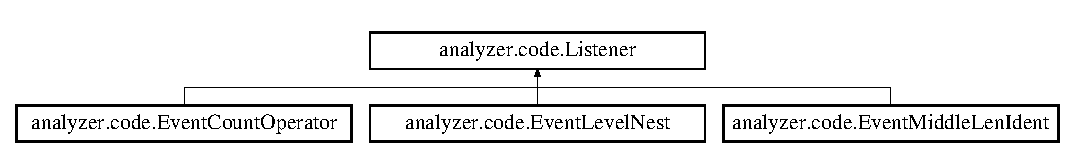
\includegraphics[height=1.674140cm]{classanalyzer_1_1code_1_1Listener}
\end{center}
\end{figure}
\subsection*{Public Member Functions}
\begin{DoxyCompactItemize}
\item 
\mbox{\Hypertarget{classanalyzer_1_1code_1_1Listener_aff4550544f22a596b50831e8c9a7e549}\label{classanalyzer_1_1code_1_1Listener_aff4550544f22a596b50831e8c9a7e549}} 
abstract void {\bfseries on\+Event} (\hyperlink{classanalyzer_1_1code_1_1Event}{Event} event)
\end{DoxyCompactItemize}


\subsection{Detailed Description}
\begin{DoxyAuthor}{Author}
tigler 
\end{DoxyAuthor}


The documentation for this class was generated from the following file\+:\begin{DoxyCompactItemize}
\item 
/home/tigler/\+Net\+Beans\+Projects/\+Plagiat/src/analyzer/code/Listener.\+java\end{DoxyCompactItemize}

\hypertarget{classanalyzer_1_1code_1_1MetricSetting}{}\section{analyzer.\+code.\+Metric\+Setting Class Reference}
\label{classanalyzer_1_1code_1_1MetricSetting}\index{analyzer.\+code.\+Metric\+Setting@{analyzer.\+code.\+Metric\+Setting}}
\subsection*{Public Member Functions}
\begin{DoxyCompactItemize}
\item 
\mbox{\Hypertarget{classanalyzer_1_1code_1_1MetricSetting_a3d0ddc8a14d995bf74f1d0911071d433}\label{classanalyzer_1_1code_1_1MetricSetting_a3d0ddc8a14d995bf74f1d0911071d433}} 
{\bfseries Metric\+Setting} (String name\+Metric, double min, double max)
\item 
\mbox{\Hypertarget{classanalyzer_1_1code_1_1MetricSetting_a47ab40bf519dd6f0ac01d22637f37fd6}\label{classanalyzer_1_1code_1_1MetricSetting_a47ab40bf519dd6f0ac01d22637f37fd6}} 
String {\bfseries get\+Name\+Metric} ()
\item 
\mbox{\Hypertarget{classanalyzer_1_1code_1_1MetricSetting_ac3bd69cf9abd575fa3c457b3076a0279}\label{classanalyzer_1_1code_1_1MetricSetting_ac3bd69cf9abd575fa3c457b3076a0279}} 
double {\bfseries get\+Min} ()
\item 
\mbox{\Hypertarget{classanalyzer_1_1code_1_1MetricSetting_a1b8e3d27c760d4ab665ce757e2d0992d}\label{classanalyzer_1_1code_1_1MetricSetting_a1b8e3d27c760d4ab665ce757e2d0992d}} 
double {\bfseries get\+Max} ()
\item 
\mbox{\Hypertarget{classanalyzer_1_1code_1_1MetricSetting_ad60c19d21233c834dffa2cdd4470b198}\label{classanalyzer_1_1code_1_1MetricSetting_ad60c19d21233c834dffa2cdd4470b198}} 
void {\bfseries set\+Name\+Metric} (String name\+Metric)
\item 
\mbox{\Hypertarget{classanalyzer_1_1code_1_1MetricSetting_ad38e9bae0dc21c88b0343f968de255fd}\label{classanalyzer_1_1code_1_1MetricSetting_ad38e9bae0dc21c88b0343f968de255fd}} 
void {\bfseries set\+Min} (double min)
\item 
\mbox{\Hypertarget{classanalyzer_1_1code_1_1MetricSetting_a2b3347cd21f8f8f40b065befaa1081b4}\label{classanalyzer_1_1code_1_1MetricSetting_a2b3347cd21f8f8f40b065befaa1081b4}} 
void {\bfseries set\+Max} (double max)
\end{DoxyCompactItemize}


\subsection{Detailed Description}
\begin{DoxyAuthor}{Author}
tigler 
\end{DoxyAuthor}


The documentation for this class was generated from the following file\+:\begin{DoxyCompactItemize}
\item 
/home/tigler/\+Net\+Beans\+Projects/\+Plagiat/src/analyzer/code/Metric\+Setting.\+java\end{DoxyCompactItemize}

\hypertarget{classanalyzer_1_1code_1_1MiddleLenIdent}{}\section{analyzer.\+code.\+Middle\+Len\+Ident Class Reference}
\label{classanalyzer_1_1code_1_1MiddleLenIdent}\index{analyzer.\+code.\+Middle\+Len\+Ident@{analyzer.\+code.\+Middle\+Len\+Ident}}
Inheritance diagram for analyzer.\+code.\+Middle\+Len\+Ident\+:\begin{figure}[H]
\begin{center}
\leavevmode
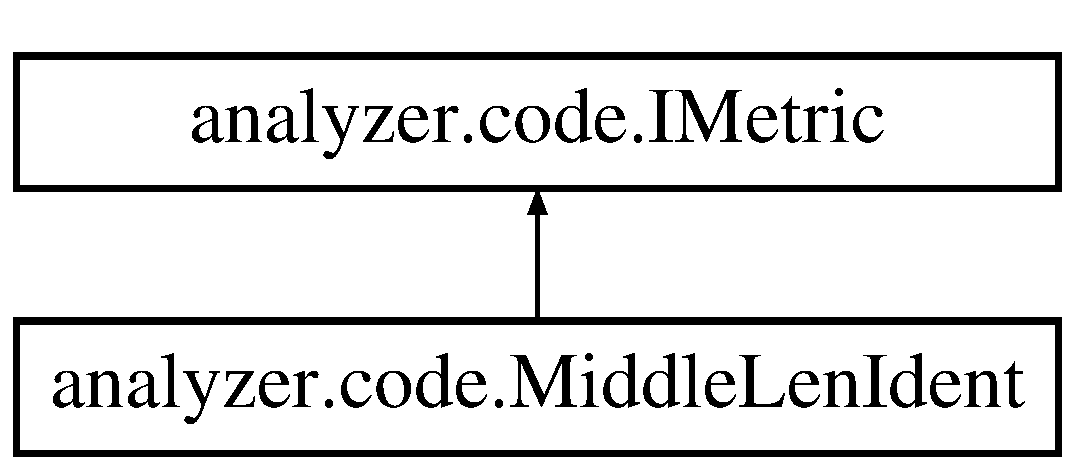
\includegraphics[height=2.000000cm]{classanalyzer_1_1code_1_1MiddleLenIdent}
\end{center}
\end{figure}
\subsection*{Public Member Functions}
\begin{DoxyCompactItemize}
\item 
\hyperlink{classanalyzer_1_1code_1_1MiddleLenIdent_a213f80eaaa3184f332af26ac940eed65}{Middle\+Len\+Ident} ()
\item 
void \hyperlink{classanalyzer_1_1code_1_1MiddleLenIdent_a8cdcf24eba4d3db76e9483ffaa2b6ea3}{calculate} (\hyperlink{classanalyzer_1_1code_1_1Event}{Event} event)
\item 
double \hyperlink{classanalyzer_1_1code_1_1MiddleLenIdent_a46411e2d526efa424d894a7b5c950625}{get\+Result} ()
\item 
void \hyperlink{classanalyzer_1_1code_1_1MiddleLenIdent_ac88413fab29f0d35a48e32c3471eb82b}{reset} ()
\end{DoxyCompactItemize}
\subsection*{Static Public Member Functions}
\begin{DoxyCompactItemize}
\item 
static String \hyperlink{classanalyzer_1_1code_1_1MiddleLenIdent_a4416bc43e60c97f489cccc3e6e9b67b1}{get\+Name} ()
\end{DoxyCompactItemize}


\subsection{Detailed Description}
Вычисляет среднюю длину идентификаторов \begin{DoxyAuthor}{Author}
tigler 
\end{DoxyAuthor}


\subsection{Constructor \& Destructor Documentation}
\mbox{\Hypertarget{classanalyzer_1_1code_1_1MiddleLenIdent_a213f80eaaa3184f332af26ac940eed65}\label{classanalyzer_1_1code_1_1MiddleLenIdent_a213f80eaaa3184f332af26ac940eed65}} 
\index{analyzer\+::code\+::\+Middle\+Len\+Ident@{analyzer\+::code\+::\+Middle\+Len\+Ident}!Middle\+Len\+Ident@{Middle\+Len\+Ident}}
\index{Middle\+Len\+Ident@{Middle\+Len\+Ident}!analyzer\+::code\+::\+Middle\+Len\+Ident@{analyzer\+::code\+::\+Middle\+Len\+Ident}}
\subsubsection{\texorpdfstring{Middle\+Len\+Ident()}{MiddleLenIdent()}}
{\footnotesize\ttfamily analyzer.\+code.\+Middle\+Len\+Ident.\+Middle\+Len\+Ident (\begin{DoxyParamCaption}{ }\end{DoxyParamCaption})\hspace{0.3cm}{\ttfamily [inline]}}

Конструктор без параметров, иницианилизирует переменные. 

\subsection{Member Function Documentation}
\mbox{\Hypertarget{classanalyzer_1_1code_1_1MiddleLenIdent_a8cdcf24eba4d3db76e9483ffaa2b6ea3}\label{classanalyzer_1_1code_1_1MiddleLenIdent_a8cdcf24eba4d3db76e9483ffaa2b6ea3}} 
\index{analyzer\+::code\+::\+Middle\+Len\+Ident@{analyzer\+::code\+::\+Middle\+Len\+Ident}!calculate@{calculate}}
\index{calculate@{calculate}!analyzer\+::code\+::\+Middle\+Len\+Ident@{analyzer\+::code\+::\+Middle\+Len\+Ident}}
\subsubsection{\texorpdfstring{calculate()}{calculate()}}
{\footnotesize\ttfamily void analyzer.\+code.\+Middle\+Len\+Ident.\+calculate (\begin{DoxyParamCaption}\item[{\hyperlink{classanalyzer_1_1code_1_1Event}{Event}}]{event }\end{DoxyParamCaption})\hspace{0.3cm}{\ttfamily [inline]}}

Суммирует длинну идентификаторов 
\begin{DoxyParams}{Parameters}
{\em event} & -\/ событие возникшее в синтаксическом анализаторе \\
\hline
\end{DoxyParams}


Implements \hyperlink{interfaceanalyzer_1_1code_1_1IMetric}{analyzer.\+code.\+I\+Metric}.

\mbox{\Hypertarget{classanalyzer_1_1code_1_1MiddleLenIdent_a4416bc43e60c97f489cccc3e6e9b67b1}\label{classanalyzer_1_1code_1_1MiddleLenIdent_a4416bc43e60c97f489cccc3e6e9b67b1}} 
\index{analyzer\+::code\+::\+Middle\+Len\+Ident@{analyzer\+::code\+::\+Middle\+Len\+Ident}!get\+Name@{get\+Name}}
\index{get\+Name@{get\+Name}!analyzer\+::code\+::\+Middle\+Len\+Ident@{analyzer\+::code\+::\+Middle\+Len\+Ident}}
\subsubsection{\texorpdfstring{get\+Name()}{getName()}}
{\footnotesize\ttfamily static String analyzer.\+code.\+Middle\+Len\+Ident.\+get\+Name (\begin{DoxyParamCaption}{ }\end{DoxyParamCaption})\hspace{0.3cm}{\ttfamily [inline]}, {\ttfamily [static]}}

Статический метод для получения названия метрики. Использует перечисление \hyperlink{enumanalyzer_1_1code_1_1EnumNamesMetric}{Enum\+Names\+Metric} с названиями метрик. \begin{DoxyReturn}{Returns}
Строку -\/ навание метрики. 
\end{DoxyReturn}
\mbox{\Hypertarget{classanalyzer_1_1code_1_1MiddleLenIdent_a46411e2d526efa424d894a7b5c950625}\label{classanalyzer_1_1code_1_1MiddleLenIdent_a46411e2d526efa424d894a7b5c950625}} 
\index{analyzer\+::code\+::\+Middle\+Len\+Ident@{analyzer\+::code\+::\+Middle\+Len\+Ident}!get\+Result@{get\+Result}}
\index{get\+Result@{get\+Result}!analyzer\+::code\+::\+Middle\+Len\+Ident@{analyzer\+::code\+::\+Middle\+Len\+Ident}}
\subsubsection{\texorpdfstring{get\+Result()}{getResult()}}
{\footnotesize\ttfamily double analyzer.\+code.\+Middle\+Len\+Ident.\+get\+Result (\begin{DoxyParamCaption}{ }\end{DoxyParamCaption})\hspace{0.3cm}{\ttfamily [inline]}}

Вычисляет среднюю длину идентификаторов \begin{DoxyReturn}{Returns}
Среднюю длину идентификаторов 
\end{DoxyReturn}


Implements \hyperlink{interfaceanalyzer_1_1code_1_1IMetric}{analyzer.\+code.\+I\+Metric}.

\mbox{\Hypertarget{classanalyzer_1_1code_1_1MiddleLenIdent_ac88413fab29f0d35a48e32c3471eb82b}\label{classanalyzer_1_1code_1_1MiddleLenIdent_ac88413fab29f0d35a48e32c3471eb82b}} 
\index{analyzer\+::code\+::\+Middle\+Len\+Ident@{analyzer\+::code\+::\+Middle\+Len\+Ident}!reset@{reset}}
\index{reset@{reset}!analyzer\+::code\+::\+Middle\+Len\+Ident@{analyzer\+::code\+::\+Middle\+Len\+Ident}}
\subsubsection{\texorpdfstring{reset()}{reset()}}
{\footnotesize\ttfamily void analyzer.\+code.\+Middle\+Len\+Ident.\+reset (\begin{DoxyParamCaption}{ }\end{DoxyParamCaption})\hspace{0.3cm}{\ttfamily [inline]}}

cбрасывает значения переменных до начальных 

Implements \hyperlink{interfaceanalyzer_1_1code_1_1IMetric}{analyzer.\+code.\+I\+Metric}.



The documentation for this class was generated from the following file\+:\begin{DoxyCompactItemize}
\item 
/home/tigler/\+Net\+Beans\+Projects/\+Plagiat/src/analyzer/code/Middle\+Len\+Ident.\+java\end{DoxyCompactItemize}

\hypertarget{classanalyzer_1_1code_1_1Scaner}{}\section{analyzer.\+code.\+Scaner Class Reference}
\label{classanalyzer_1_1code_1_1Scaner}\index{analyzer.\+code.\+Scaner@{analyzer.\+code.\+Scaner}}
Inheritance diagram for analyzer.\+code.\+Scaner\+:\begin{figure}[H]
\begin{center}
\leavevmode
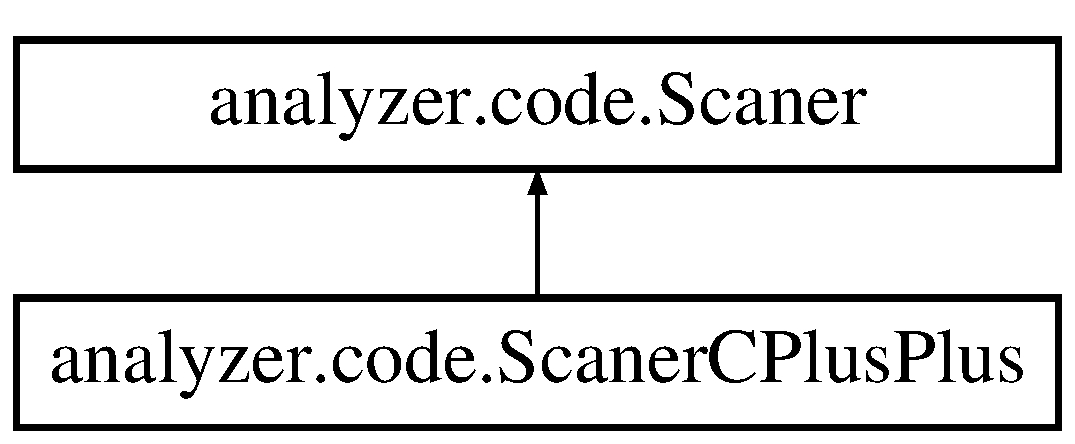
\includegraphics[height=2.000000cm]{classanalyzer_1_1code_1_1Scaner}
\end{center}
\end{figure}
\subsection*{Public Member Functions}
\begin{DoxyCompactItemize}
\item 
\mbox{\Hypertarget{classanalyzer_1_1code_1_1Scaner_ae8ef99f07981cdc050db2ac72b87764c}\label{classanalyzer_1_1code_1_1Scaner_ae8ef99f07981cdc050db2ac72b87764c}} 
abstract \hyperlink{classanalyzer_1_1code_1_1Lexem}{Lexem} {\bfseries Scan} ()
\item 
\mbox{\Hypertarget{classanalyzer_1_1code_1_1Scaner_aa0eead1a1a7e0b57b974fdd82b3ff994}\label{classanalyzer_1_1code_1_1Scaner_aa0eead1a1a7e0b57b974fdd82b3ff994}} 
abstract int {\bfseries Get\+UK} ()
\item 
\mbox{\Hypertarget{classanalyzer_1_1code_1_1Scaner_a3715352096865139df63d8392c77541f}\label{classanalyzer_1_1code_1_1Scaner_a3715352096865139df63d8392c77541f}} 
abstract void {\bfseries Put\+UK} (int uk)
\item 
\mbox{\Hypertarget{classanalyzer_1_1code_1_1Scaner_a868b7448acbe6444ad9bd326949effb1}\label{classanalyzer_1_1code_1_1Scaner_a868b7448acbe6444ad9bd326949effb1}} 
abstract void {\bfseries Print\+Error} (String err, String a, int str)
\end{DoxyCompactItemize}
\subsection*{Protected Attributes}
\begin{DoxyCompactItemize}
\item 
\mbox{\Hypertarget{classanalyzer_1_1code_1_1Scaner_af22f29cc210b51910a21d62c6b03ea62}\label{classanalyzer_1_1code_1_1Scaner_af22f29cc210b51910a21d62c6b03ea62}} 
String {\bfseries t}
\item 
\mbox{\Hypertarget{classanalyzer_1_1code_1_1Scaner_ac32aa31f770456bc608c79d1b413560d}\label{classanalyzer_1_1code_1_1Scaner_ac32aa31f770456bc608c79d1b413560d}} 
int {\bfseries uk}
\item 
\mbox{\Hypertarget{classanalyzer_1_1code_1_1Scaner_a1c252e1e16eaa8b59aadc78e7d775f45}\label{classanalyzer_1_1code_1_1Scaner_a1c252e1e16eaa8b59aadc78e7d775f45}} 
int {\bfseries str}
\item 
\mbox{\Hypertarget{classanalyzer_1_1code_1_1Scaner_a64c17378be4c913299fd855b489f3a0a}\label{classanalyzer_1_1code_1_1Scaner_a64c17378be4c913299fd855b489f3a0a}} 
int {\bfseries stl}
\end{DoxyCompactItemize}


\subsection{Detailed Description}
\begin{DoxyAuthor}{Author}
tigler 
\end{DoxyAuthor}


The documentation for this class was generated from the following file\+:\begin{DoxyCompactItemize}
\item 
/home/tigler/\+Net\+Beans\+Projects/\+Plagiat/src/analyzer/code/Scaner.\+java\end{DoxyCompactItemize}

\hypertarget{classanalyzer_1_1code_1_1ScanerCPlusPlus}{}\section{analyzer.\+code.\+Scaner\+C\+Plus\+Plus Class Reference}
\label{classanalyzer_1_1code_1_1ScanerCPlusPlus}\index{analyzer.\+code.\+Scaner\+C\+Plus\+Plus@{analyzer.\+code.\+Scaner\+C\+Plus\+Plus}}
Inheritance diagram for analyzer.\+code.\+Scaner\+C\+Plus\+Plus\+:\begin{figure}[H]
\begin{center}
\leavevmode
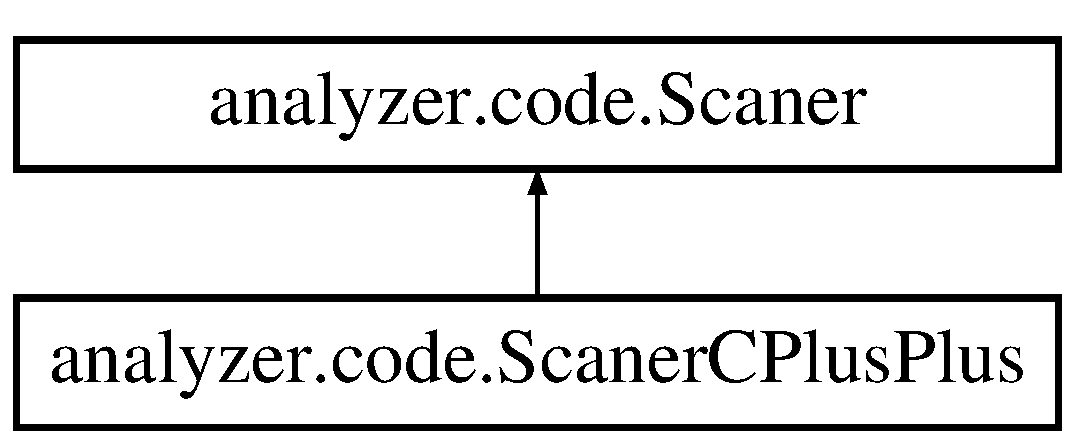
\includegraphics[height=2.000000cm]{classanalyzer_1_1code_1_1ScanerCPlusPlus}
\end{center}
\end{figure}
\subsection*{Public Member Functions}
\begin{DoxyCompactItemize}
\item 
\mbox{\Hypertarget{classanalyzer_1_1code_1_1ScanerCPlusPlus_a8e206ebf05aeda8102ed5993e8e699c4}\label{classanalyzer_1_1code_1_1ScanerCPlusPlus_a8e206ebf05aeda8102ed5993e8e699c4}} 
\hyperlink{classanalyzer_1_1code_1_1Lexem}{Lexem} {\bfseries Scan} ()
\item 
\mbox{\Hypertarget{classanalyzer_1_1code_1_1ScanerCPlusPlus_a7920424438e26e69853c7486051e6f7b}\label{classanalyzer_1_1code_1_1ScanerCPlusPlus_a7920424438e26e69853c7486051e6f7b}} 
{\bfseries Scaner\+C\+Plus\+Plus} (String text)
\item 
\mbox{\Hypertarget{classanalyzer_1_1code_1_1ScanerCPlusPlus_a0723d812bda76c14824fcce55059e662}\label{classanalyzer_1_1code_1_1ScanerCPlusPlus_a0723d812bda76c14824fcce55059e662}} 
int {\bfseries Get\+UK} ()
\item 
\mbox{\Hypertarget{classanalyzer_1_1code_1_1ScanerCPlusPlus_aa3d7eaf52f3523a16726bded0428d124}\label{classanalyzer_1_1code_1_1ScanerCPlusPlus_aa3d7eaf52f3523a16726bded0428d124}} 
void {\bfseries Put\+UK} (int auk)
\item 
\mbox{\Hypertarget{classanalyzer_1_1code_1_1ScanerCPlusPlus_a4368151d61a92ae270dbe119bab21ef6}\label{classanalyzer_1_1code_1_1ScanerCPlusPlus_a4368151d61a92ae270dbe119bab21ef6}} 
void {\bfseries Print\+Error} (String err, String a, int str)
\end{DoxyCompactItemize}
\subsection*{Additional Inherited Members}


\subsection{Detailed Description}
\begin{DoxyAuthor}{Author}
tigler 
\end{DoxyAuthor}


The documentation for this class was generated from the following file\+:\begin{DoxyCompactItemize}
\item 
/home/tigler/\+Net\+Beans\+Projects/\+Plagiat/src/analyzer/code/Scaner\+C\+Plus\+Plus.\+java\end{DoxyCompactItemize}

\hypertarget{classanalyzer_1_1code_1_1SyntaxAnalyzer}{}\section{analyzer.\+code.\+Syntax\+Analyzer Class Reference}
\label{classanalyzer_1_1code_1_1SyntaxAnalyzer}\index{analyzer.\+code.\+Syntax\+Analyzer@{analyzer.\+code.\+Syntax\+Analyzer}}
Inheritance diagram for analyzer.\+code.\+Syntax\+Analyzer\+:\begin{figure}[H]
\begin{center}
\leavevmode
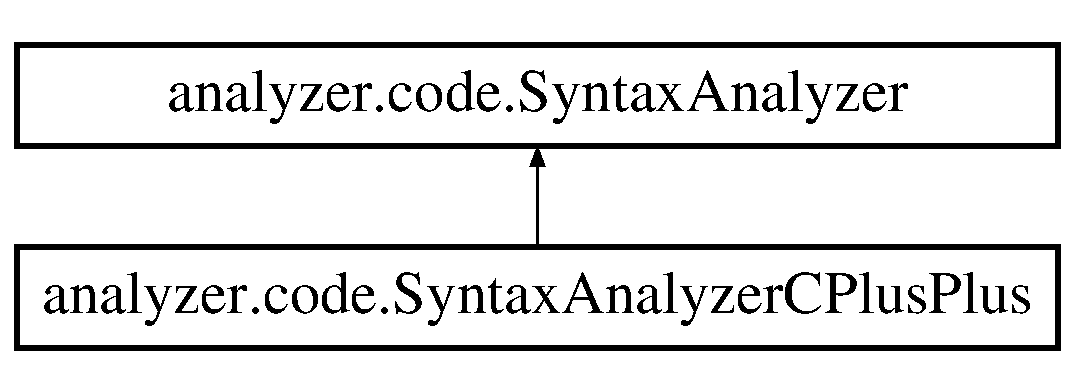
\includegraphics[height=2.000000cm]{classanalyzer_1_1code_1_1SyntaxAnalyzer}
\end{center}
\end{figure}
\subsection*{Public Member Functions}
\begin{DoxyCompactItemize}
\item 
\mbox{\Hypertarget{classanalyzer_1_1code_1_1SyntaxAnalyzer_a77000f1752e71019a73c2da546510d91}\label{classanalyzer_1_1code_1_1SyntaxAnalyzer_a77000f1752e71019a73c2da546510d91}} 
abstract void {\bfseries attach} (\hyperlink{classanalyzer_1_1code_1_1Listener}{Listener} listener)
\item 
\mbox{\Hypertarget{classanalyzer_1_1code_1_1SyntaxAnalyzer_a5e23e6a26a8931dfdc6b356f73fb1260}\label{classanalyzer_1_1code_1_1SyntaxAnalyzer_a5e23e6a26a8931dfdc6b356f73fb1260}} 
abstract void {\bfseries start} ()
\item 
\mbox{\Hypertarget{classanalyzer_1_1code_1_1SyntaxAnalyzer_ab928134f83adb33bf380ee5f41f27370}\label{classanalyzer_1_1code_1_1SyntaxAnalyzer_ab928134f83adb33bf380ee5f41f27370}} 
abstract void {\bfseries set\+Text} (String text)
\end{DoxyCompactItemize}
\subsection*{Protected Attributes}
\begin{DoxyCompactItemize}
\item 
\mbox{\Hypertarget{classanalyzer_1_1code_1_1SyntaxAnalyzer_af2fdfde9049c0b9d77d8bbacc5a67496}\label{classanalyzer_1_1code_1_1SyntaxAnalyzer_af2fdfde9049c0b9d77d8bbacc5a67496}} 
\hyperlink{classanalyzer_1_1code_1_1Scaner}{Scaner} {\bfseries sc}
\item 
\mbox{\Hypertarget{classanalyzer_1_1code_1_1SyntaxAnalyzer_a8aceea502e1f902fbd3200f0a514d536}\label{classanalyzer_1_1code_1_1SyntaxAnalyzer_a8aceea502e1f902fbd3200f0a514d536}} 
String {\bfseries text}
\item 
\mbox{\Hypertarget{classanalyzer_1_1code_1_1SyntaxAnalyzer_a48ccf4c34b0824b9463924ac99f76bc5}\label{classanalyzer_1_1code_1_1SyntaxAnalyzer_a48ccf4c34b0824b9463924ac99f76bc5}} 
\hyperlink{classanalyzer_1_1code_1_1Listener}{Listener} {\bfseries listener}
\end{DoxyCompactItemize}


\subsection{Detailed Description}
\begin{DoxyAuthor}{Author}
tigler 
\end{DoxyAuthor}


The documentation for this class was generated from the following file\+:\begin{DoxyCompactItemize}
\item 
/home/tigler/\+Net\+Beans\+Projects/\+Plagiat/src/analyzer/code/Syntax\+Analyzer.\+java\end{DoxyCompactItemize}

\hypertarget{classanalyzer_1_1code_1_1SyntaxAnalyzerCPlusPlus}{}\section{analyzer.\+code.\+Syntax\+Analyzer\+C\+Plus\+Plus Class Reference}
\label{classanalyzer_1_1code_1_1SyntaxAnalyzerCPlusPlus}\index{analyzer.\+code.\+Syntax\+Analyzer\+C\+Plus\+Plus@{analyzer.\+code.\+Syntax\+Analyzer\+C\+Plus\+Plus}}
Inheritance diagram for analyzer.\+code.\+Syntax\+Analyzer\+C\+Plus\+Plus\+:\begin{figure}[H]
\begin{center}
\leavevmode
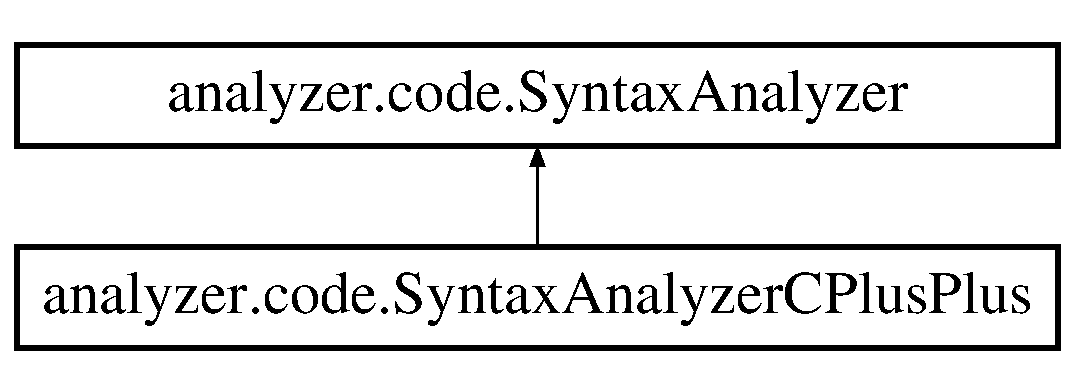
\includegraphics[height=2.000000cm]{classanalyzer_1_1code_1_1SyntaxAnalyzerCPlusPlus}
\end{center}
\end{figure}
\subsection*{Public Member Functions}
\begin{DoxyCompactItemize}
\item 
\mbox{\Hypertarget{classanalyzer_1_1code_1_1SyntaxAnalyzerCPlusPlus_a62ecabba5c6989ef558f0a991b3798a7}\label{classanalyzer_1_1code_1_1SyntaxAnalyzerCPlusPlus_a62ecabba5c6989ef558f0a991b3798a7}} 
{\bfseries Syntax\+Analyzer\+C\+Plus\+Plus} (String text)
\item 
\mbox{\Hypertarget{classanalyzer_1_1code_1_1SyntaxAnalyzerCPlusPlus_ab687e2baba100eb38b3e0df3f68a2927}\label{classanalyzer_1_1code_1_1SyntaxAnalyzerCPlusPlus_ab687e2baba100eb38b3e0df3f68a2927}} 
void {\bfseries set\+Text} (String text)
\item 
\mbox{\Hypertarget{classanalyzer_1_1code_1_1SyntaxAnalyzerCPlusPlus_ac016b5fa6a0eef248a16601c940af7a8}\label{classanalyzer_1_1code_1_1SyntaxAnalyzerCPlusPlus_ac016b5fa6a0eef248a16601c940af7a8}} 
void {\bfseries attach} (\hyperlink{classanalyzer_1_1code_1_1Listener}{Listener} listener)
\item 
\mbox{\Hypertarget{classanalyzer_1_1code_1_1SyntaxAnalyzerCPlusPlus_a09c25e5223e8fd584b3bc01da4da8dc1}\label{classanalyzer_1_1code_1_1SyntaxAnalyzerCPlusPlus_a09c25e5223e8fd584b3bc01da4da8dc1}} 
void {\bfseries start} ()
\item 
\mbox{\Hypertarget{classanalyzer_1_1code_1_1SyntaxAnalyzerCPlusPlus_a1f158c1f95c1835f4f0d6613d907bfe5}\label{classanalyzer_1_1code_1_1SyntaxAnalyzerCPlusPlus_a1f158c1f95c1835f4f0d6613d907bfe5}} 
void {\bfseries Axiom} ()
\item 
\mbox{\Hypertarget{classanalyzer_1_1code_1_1SyntaxAnalyzerCPlusPlus_af226bd1ed332b7b5657dca919246ee46}\label{classanalyzer_1_1code_1_1SyntaxAnalyzerCPlusPlus_af226bd1ed332b7b5657dca919246ee46}} 
void {\bfseries IF} ()
\end{DoxyCompactItemize}
\subsection*{Additional Inherited Members}


\subsection{Detailed Description}
\begin{DoxyAuthor}{Author}
tigler 
\end{DoxyAuthor}


The documentation for this class was generated from the following file\+:\begin{DoxyCompactItemize}
\item 
/home/tigler/\+Net\+Beans\+Projects/\+Plagiat/src/analyzer/code/Syntax\+Analyzer\+C\+Plus\+Plus.\+java\end{DoxyCompactItemize}

\hypertarget{classanalyzer_1_1code_1_1Unknown}{}\section{analyzer.\+code.\+Unknown Class Reference}
\label{classanalyzer_1_1code_1_1Unknown}\index{analyzer.\+code.\+Unknown@{analyzer.\+code.\+Unknown}}
\subsection*{Public Member Functions}
\begin{DoxyCompactItemize}
\item 
\hyperlink{classanalyzer_1_1code_1_1Unknown_a4ff369156174790c6388be27c0e56bef}{Unknown} ()
\item 
void \hyperlink{classanalyzer_1_1code_1_1Unknown_a7229e15dc0bba3a32526b47cf55e5e1e}{set\+Error} (String err)
\end{DoxyCompactItemize}


\subsection{Detailed Description}
Используется для скопления нераспознанных лексем \begin{DoxyAuthor}{Author}
tigler 
\end{DoxyAuthor}


\subsection{Constructor \& Destructor Documentation}
\mbox{\Hypertarget{classanalyzer_1_1code_1_1Unknown_a4ff369156174790c6388be27c0e56bef}\label{classanalyzer_1_1code_1_1Unknown_a4ff369156174790c6388be27c0e56bef}} 
\index{analyzer\+::code\+::\+Unknown@{analyzer\+::code\+::\+Unknown}!Unknown@{Unknown}}
\index{Unknown@{Unknown}!analyzer\+::code\+::\+Unknown@{analyzer\+::code\+::\+Unknown}}
\subsubsection{\texorpdfstring{Unknown()}{Unknown()}}
{\footnotesize\ttfamily analyzer.\+code.\+Unknown.\+Unknown (\begin{DoxyParamCaption}{ }\end{DoxyParamCaption})\hspace{0.3cm}{\ttfamily [inline]}}

Конструктор без параметров, инициализирует контейнер для неизвестных лексем 

\subsection{Member Function Documentation}
\mbox{\Hypertarget{classanalyzer_1_1code_1_1Unknown_a7229e15dc0bba3a32526b47cf55e5e1e}\label{classanalyzer_1_1code_1_1Unknown_a7229e15dc0bba3a32526b47cf55e5e1e}} 
\index{analyzer\+::code\+::\+Unknown@{analyzer\+::code\+::\+Unknown}!set\+Error@{set\+Error}}
\index{set\+Error@{set\+Error}!analyzer\+::code\+::\+Unknown@{analyzer\+::code\+::\+Unknown}}
\subsubsection{\texorpdfstring{set\+Error()}{setError()}}
{\footnotesize\ttfamily void analyzer.\+code.\+Unknown.\+set\+Error (\begin{DoxyParamCaption}\item[{String}]{err }\end{DoxyParamCaption})\hspace{0.3cm}{\ttfamily [inline]}}

Запомнить неизвестную лексемму 
\begin{DoxyParams}{Parameters}
{\em err} & -\/ Строка -\/ вносимая лексема. \\
\hline
\end{DoxyParams}


The documentation for this class was generated from the following file\+:\begin{DoxyCompactItemize}
\item 
/home/tigler/\+Net\+Beans\+Projects/\+Plagiat/src/analyzer/code/Unknown.\+java\end{DoxyCompactItemize}

\hypertarget{classanalyzer_1_1code_1_1Variable}{}\section{analyzer.\+code.\+Variable Class Reference}
\label{classanalyzer_1_1code_1_1Variable}\index{analyzer.\+code.\+Variable@{analyzer.\+code.\+Variable}}
\subsection*{Public Member Functions}
\begin{DoxyCompactItemize}
\item 
\hyperlink{classanalyzer_1_1code_1_1Variable_a492abfcee26b2bf104175ff2772c3a76}{Variable} (String ident)
\item 
void \hyperlink{classanalyzer_1_1code_1_1Variable_a9ff60aa209b91fd406d2f529fd4d721d}{inc\+Count\+Operators} ()
\item 
int \hyperlink{classanalyzer_1_1code_1_1Variable_a03cf6dacfd545ab3ee82b5109ecd0e14}{get\+Count\+Operators} ()
\end{DoxyCompactItemize}


\subsection{Detailed Description}
Опеределяет переменную, в исходном коде. \begin{DoxyAuthor}{Author}
tigler 
\end{DoxyAuthor}


\subsection{Constructor \& Destructor Documentation}
\mbox{\Hypertarget{classanalyzer_1_1code_1_1Variable_a492abfcee26b2bf104175ff2772c3a76}\label{classanalyzer_1_1code_1_1Variable_a492abfcee26b2bf104175ff2772c3a76}} 
\index{analyzer\+::code\+::\+Variable@{analyzer\+::code\+::\+Variable}!Variable@{Variable}}
\index{Variable@{Variable}!analyzer\+::code\+::\+Variable@{analyzer\+::code\+::\+Variable}}
\subsubsection{\texorpdfstring{Variable()}{Variable()}}
{\footnotesize\ttfamily analyzer.\+code.\+Variable.\+Variable (\begin{DoxyParamCaption}\item[{String}]{ident }\end{DoxyParamCaption})\hspace{0.3cm}{\ttfamily [inline]}}

Конструктор с параметром 
\begin{DoxyParams}{Parameters}
{\em ident} & -\/ Строка -\/ идентификатор переменной. \\
\hline
\end{DoxyParams}


\subsection{Member Function Documentation}
\mbox{\Hypertarget{classanalyzer_1_1code_1_1Variable_a03cf6dacfd545ab3ee82b5109ecd0e14}\label{classanalyzer_1_1code_1_1Variable_a03cf6dacfd545ab3ee82b5109ecd0e14}} 
\index{analyzer\+::code\+::\+Variable@{analyzer\+::code\+::\+Variable}!get\+Count\+Operators@{get\+Count\+Operators}}
\index{get\+Count\+Operators@{get\+Count\+Operators}!analyzer\+::code\+::\+Variable@{analyzer\+::code\+::\+Variable}}
\subsubsection{\texorpdfstring{get\+Count\+Operators()}{getCountOperators()}}
{\footnotesize\ttfamily int analyzer.\+code.\+Variable.\+get\+Count\+Operators (\begin{DoxyParamCaption}{ }\end{DoxyParamCaption})\hspace{0.3cm}{\ttfamily [inline]}}

Получить количество операторов. \begin{DoxyReturn}{Returns}
-\/ count\+Operators 
\end{DoxyReturn}
\mbox{\Hypertarget{classanalyzer_1_1code_1_1Variable_a9ff60aa209b91fd406d2f529fd4d721d}\label{classanalyzer_1_1code_1_1Variable_a9ff60aa209b91fd406d2f529fd4d721d}} 
\index{analyzer\+::code\+::\+Variable@{analyzer\+::code\+::\+Variable}!inc\+Count\+Operators@{inc\+Count\+Operators}}
\index{inc\+Count\+Operators@{inc\+Count\+Operators}!analyzer\+::code\+::\+Variable@{analyzer\+::code\+::\+Variable}}
\subsubsection{\texorpdfstring{inc\+Count\+Operators()}{incCountOperators()}}
{\footnotesize\ttfamily void analyzer.\+code.\+Variable.\+inc\+Count\+Operators (\begin{DoxyParamCaption}{ }\end{DoxyParamCaption})\hspace{0.3cm}{\ttfamily [inline]}}

инкрементирует переменную класса count\+Operators(увеличение количества операторов) 

The documentation for this class was generated from the following file\+:\begin{DoxyCompactItemize}
\item 
/home/tigler/\+Net\+Beans\+Projects/\+Plagiat/src/analyzer/code/Variable.\+java\end{DoxyCompactItemize}

%--- End generated contents ---

% Index
\backmatter
\newpage
\phantomsection
\clearemptydoublepage
\addcontentsline{toc}{chapter}{Index}
\printindex

\end{document}
